\documentclass[11pt]{article}
\usepackage[margin=1in]{geometry}
\usepackage[T1]{fontenc}
\usepackage{lmodern}
\usepackage{amsmath,amssymb,amsthm,mathtools,mathrsfs}
\usepackage{microtype,enumitem,xcolor,tikz}
\usetikzlibrary{arrows.meta,positioning,calc,decorations.pathreplacing,patterns}
\usepackage[colorlinks=true,linkcolor=blue!45!black,citecolor=blue!45!black,urlcolor=blue!45!black]{hyperref}
\hypersetup{pdftitle={A directional zero-one law for finite-range-dependent random environments},pdfauthor={OpenAI}}
\setlength{\emergencystretch}{2em}
\setlist{itemsep=3pt,topsep=5pt}
\numberwithin{equation}{section}
\newtheorem{theorem}{Theorem}[section]
\newtheorem{proposition}[theorem]{Proposition}
\newtheorem{lemma}[theorem]{Lemma}
\newtheorem{corollary}[theorem]{Corollary}
\theoremstyle{definition}
\newtheorem{definition}[theorem]{Definition}
\theoremstyle{remark}
\newtheorem{remark}[theorem]{Remark}
\newcommand{\RR}{\mathbb R}
\newcommand{\ZZ}{\mathbb Z}
\newcommand{\EE}{\mathbb E}
\newcommand{\PP}{\mathbb P}
\newcommand{\one}{\mathbf 1}
\newcommand{\abs}[1]{\lvert #1\rvert}
\newcommand{\norm}[1]{\lVert #1\rVert}
\newcommand{\Ent}{\mathscr H}
\DeclareMathOperator{\Dep}{Dep}
\DeclareMathOperator{\dist}{dist}
\title{A directional zero--one law for\newline finite-range-dependent random environments}
\author{OpenAI}
\date{October 5, 2026}
\begin{document}
\maketitle
\begin{abstract}
We prove a directional zero--one law for uniformly elliptic nearest-neighbor
random walks in stationary, ergodic, finite-range-dependent environments on
$\ZZ^d$, $d\ge3$. For every fixed nonzero real direction, the probability
of escape in that direction, averaged over the environment, is either zero
or one. Finite-range dependence is imposed on the full transition rows:
collections of rows at distance greater than a fixed range are independent,
including collections indexed by infinite deterministic sets.
\end{abstract}

\section{Introduction}\label{sec:introduction}

A random walk in a random environment encounters the same transition
probabilities whenever it returns to a site. This persistence distinguishes
the model from a walk whose transition probabilities are resampled at each
step. Directional transience asks whether the walk eventually moves beyond
every hyperplane perpendicular to a fixed direction. The directional
zero--one question is whether this escape event can have probability
strictly between zero and one after averaging over the environment.

\subsection{Model and main theorem}

Fix $d\ge3$ and let $U=\{\pm e_1,\ldots,\pm e_d\}$ be the coordinate
unit steps. Set
\[
 \Delta_U=\left\{p\in[0,1]^U:\sum_{e\in U}p(e)=1\right\},
 \qquad \Omega=\Delta_U^{\ZZ^d},
\]
with its product Borel sigma-field. An environment $\omega\in\Omega$
assigns the row $\omega(x,\cdot)$ to each site $x$. Let $Q$ be a Borel
probability law on $\Omega$ satisfying the following assumptions.

\begin{enumerate}[label=\textup{(\roman*)}]
\item \emph{Stationarity and ergodicity.}
For $z\in\ZZ^d$, define
$(\theta_z\omega)(x,e)=\omega(x+z,e)$. The law $Q$ is invariant under
every $\theta_z$, and every event invariant modulo null sets under all
these translations has probability zero or one.
\item \emph{Uniform ellipticity.}
For some deterministic $\kappa>0$,
\[
 Q\bigl(\omega(x,e)\ge\kappa
          \text{ for every }x\in\ZZ^d,\ e\in U\bigr)=1.
\]
\item \emph{Finite-range dependence.}
For some deterministic integer $R\ge0$, the sigma-fields
\[
 \mathcal F_A=\sigma\bigl(\omega(x,e):x\in A,\ e\in U\bigr),
 \qquad \mathcal F_B=\sigma\bigl(\omega(x,e):x\in B,\ e\in U\bigr)
\]
are independent whenever the nonempty deterministic sets
$A,B\subseteq\ZZ^d$ satisfy
\begin{equation}\label{eq:finite-range}
 \dist_\infty(A,B):=
 \inf_{a\in A,\,b\in B}\norm{a-b}_\infty>R.
\end{equation}
This condition includes infinite sets.
\end{enumerate}

For fixed $\omega$, let $P_{x,\omega}$ be the law of the Markov chain
started at $x$ with transitions
\[
 P_{x,\omega}(X_{n+1}=y+e\mid X_n=y)=\omega(y,e).
\]
Its annealed law is $P_x=\int P_{x,\omega}\,Q(d\omega)$.
For each fixed $\ell\in\RR^d\setminus\{0\}$, write
\[
 A_\ell=\{X_n\cdot\ell\longrightarrow+\infty\}.
\]

\begin{theorem}[Directional zero--one law]\label{thm:main}
Under assumptions \textup{(i)--(iii)}, for every fixed
$\ell\in\RR^d\setminus\{0\}$,
\[
 P_0(A_\ell)\in\{0,1\}.
\]
\end{theorem}

The dependence range and ellipticity constant may vary with the law $Q$.
The direction may be irrational; it is fixed before taking probability.
The proof uses stationarity and finite-range independence directly, without
an additional appeal to ergodicity. Its independence arguments concern
separated sigma-fields of rows, rather than any representation of the
environment in terms of independent labels.

\subsection{Background and relation to earlier work}

Directional zero--one laws are a basic part of the transience theory of
random walks in random environments. Kalikow's work
\cite{Kalikow1981}, together with the regeneration formulation of
Sznitman and Zerner \cite[Lemma~1.1]{SznitmanZerner1999}, established
the sign-union law for uniformly elliptic iid environments,
\[
 P_0(A_\ell\cup A_{-\ell})\in\{0,1\}.
\]
This leaves open which sign is chosen when the union has probability
one. In two dimensions, Zerner and Merkl \cite{ZernerMerkl2001}
proved the full directional zero--one law for iid elliptic environments;
Zerner \cite{Zerner2007} subsequently gave a revised proof. The planar
arguments exploit intersections of paths. The question in higher
dimensions requires a different way to exclude two possible escape signs.

Regeneration is a central tool for this problem and for laws of large
numbers. Sznitman and Zerner
\cite[Theorem~1.4 and Corollary~1.5]{SznitmanZerner1999} constructed
independent increments after suitable record times in an iid environment.
Results on asymptotic directions further distinguish a deterministic
axis from the choice of a sign on that axis: see Simenhaus
\cite{Simenhaus2007} and Drewitz and Ram\'irez
\cite{DrewitzRamirez2010}. A limiting direction or a conditional law of
large numbers does not by itself establish a directional zero--one law.

For dependent environments, Comets and Zeitouni
\cite{CometsZeitouni2004} used environment-independent forced steps to
construct approximate regeneration under mixing assumptions, with
additional hypotheses yielding a law of large numbers. That forcing
device is an antecedent of the marked scripts used here. Rassoul-Agha
\cite{RassoulAgha2005} derived a law of large numbers under Gibbs mixing
assumptions and a directional zero--one hypothesis. Guo
\cite{Guo2014} proved conditional velocity results under a mixing
condition that includes finite-range-dependent environments. These
conclusions concern velocity and do not determine the probabilities of
the two directional escape events. Exact finite-range independence is
also stronger than decay of local correlations: Bramson, Zeitouni, and
Zerner \cite[Theorem~3]{BramsonZeitouniZerner2006} constructed stationary,
uniformly elliptic, polynomially mixing environments in dimension at
least three with positive probability of escape in each of two opposite
directions.

The companion article \cite[Theorem~1.1]{OpenAI2026} proves the iid
directional zero--one law under strict ellipticity: every transition
probability is positive, but no uniform lower bound is required. Here we
extend the uniformly elliptic case to finite-range dependence. The proof
adapts the radius-and-contact strategy developed in
\cite[Sections~2--7]{OpenAI2026}. In that strategy, coexistence first
forces integrability of spatial regeneration radii. Two independent
sequences of regeneration pieces are then placed in an opposed arrangement,
and entropy and endpoint-posterior estimates give incompatible bounds on
their contacts. We retain this architecture and prove all required
estimates for the present environment law. The finite-range extension
depends on keeping track of the rows actually used by a marked path,
replacing intersections by proximity within the dependence range, and
transferring only the stopped path laws justified by separated rows.
No conditional density assumption, independent-label representation,
positive speed, or moment bound on regeneration times is imposed.


\subsection{Proof strategy and additional ingredients}

The argument rules out coexistence of escape in opposite directions.
For a fixed direction, we construct independent regeneration pieces:
finite path segments ending at new record heights that the subsequent
path never undercuts. This construction proves that positive probability
of escape in that direction makes the two escape signs exhaustive.

Finite-range dependence creates two obstacles to the usual iid reasoning.
Disjoint paths can use correlated rows, and an observed path can change the
law of nearby unobserved rows. We split each transition into two marked
choices of constant weight and a remaining choice. A prescribed sequence
of the constant-weight choices moves beyond the dependence range without
using any further row information. This leaves a region of genuinely
independent rows for a continuation that stays beyond its endpoint.
The prescribed sequences cannot overlap, so the regeneration pieces have
an unambiguous concatenation law. Conditioning at their endpoints is
proved by enumeration of finite prefixes, since those endpoints are
selected using the future.

Under coexistence, the regeneration pieces have finite mean spatial
radius. The proof uses a large transverse excursion to splice in an
oppositely directed continuation, separated from the observed path by a
tilted hyperplane and a short marked connector. Repeating the construction
would place uniformly positive probability in disjoint windows for the
walk's final directional supremum. This contradiction gives the radius
bound. It yields opposite deterministic limiting rays and reduces an
arbitrary real direction to a coordinate direction.

For that coordinate, place independent positive and negative sequences
of regeneration pieces in an opposed arrangement. A contact means that
their departure sites come within distance $R$. Common regeneration
heights divide the arrangement into iid pairs of lists. Finite spatial
moments bound the entropy of their cumulative lateral displacement.
Comparing long chunks with independent bridges---concatenated regeneration
pieces conditioned on prescribed total widths---then shows that among
the first $J$ dyadic intervals of block indices, the expected number
containing a contact is $O(J/\log J)$.

The opposite estimate uses endpoint alignment. Start a negative path,
conditioned to stay below its starting height, just below a positive
bridge's endpoint, and search for their first contact along the positive
path. Posterior probabilities for a finite set of possible lateral
endpoints form a vector of martingales. The sum of their running
maxima has an exponential tail on the scale of the logarithm of the number
of endpoints. The marked segment ending an observed prefix at a lower
height permits comparison with a fresh path law up to its first exit
from a specified slab. The posterior
functions retain their original meaning; only the stopped path marginal
is transferred. Combining this estimate with nearby-point comparisons of
quenched exit probabilities forces $\Omega(J/\log\log J)$ contact scales,
contradicting the entropy bound.

The finite-range adaptations are the marked separation, killing on entry
to neighborhoods of radius $R$, and comparison of stopped posterior
processes across the resulting gaps between active rows.
We prove in full the vector-martingale estimate of
\cite[Lemma~6.1]{OpenAI2026}; it controls the cost of selecting a path
through an endpoint constraint.

Section~\ref{sec:cuts} establishes regeneration and mean widths.
Section~\ref{sec:radius} proves spatial integrability and reduces to
coordinate coexistence. Sections~\ref{sec:bridges} and~\ref{sec:entropy}
construct the opposed arrangement and its contact upper bound.
Section~\ref{sec:posteriors} proves the endpoint estimate, and
Section~\ref{sec:contact-lower} obtains the contradictory lower bound.

\section{Separated rows and regeneration words}\label{sec:cuts}

We first construct independent successive pieces of a walk that stays
above its initial level in a prescribed direction.  Finite-range dependence requires a
gap between the rows used by consecutive pieces.  We create that gap by
marking some transitions whose probabilities are constant, so that the
walk can cross the gap without using its environmental rows.  The
construction will also prove the directional sign-union statement and a
finite mean for the spatial width of each piece.  Throughout this section
the direction may be any fixed nonzero real vector.  We adapt the
regeneration and record-count arguments of
\cite[Section~2]{OpenAI2026}, proving here the separated-row identities
needed for finite-range dependence.

\subsection{Marks and the rows a path uses}

We use the same splitting device as the independent-coin construction
of Comets and Zeitouni \cite[Equation~(2.1)]{CometsZeitouni2004}:
an environment-independent choice forces a step, and a residual choice
restores the prescribed transition row.  Two distinguished marks will
also prevent overlapping occurrences of the prescribed step sequence
introduced below.

Fix \(\lambda>0\) with \(2\lambda<\kappa\).  Enlarge the walk by giving
each step a mark in \(\{0,1,*\}\).  Conditional on the environment and
the marked past, a step from \(x\) has joint probabilities
\begin{equation}\label{eq:marked-kernel}
 \begin{aligned}
 P_{x,\omega}(X_1=x+e,\text{ mark }0)&=\lambda,\\
 P_{x,\omega}(X_1=x+e,\text{ mark }1)&=\lambda,\\
 P_{x,\omega}(X_1=x+e,\text{ mark }*)&=\omega(x,e)-2\lambda,
 \qquad e\in U.
 \end{aligned}
\end{equation}
These probabilities are nonnegative and sum to one.  Summing over the
marks recovers the original transition row, so every assertion about
the unmarked path is unchanged.  We keep the notation
\(P_{x,\omega}\) and \(P_x\) for the marked quenched and annealed laws.
We call these laws \emph{raw} when no condition of staying on one side of
a barrier is imposed.  The path filtration includes both positions and
the marks of steps already taken.  All constructions take place on the
full-measure set where the ellipticity inequalities hold at every site;
the marked kernel may be defined arbitrarily elsewhere.

A finite marked word \(\gamma\) consists of positions
\(x_0,\ldots,x_t\), with \(x_{j+1}-x_j\in U\), and one mark for each
of its \(t\) steps.  Its departure set and active departure set are
\[
 \Dep(\gamma)=\{x_0,\ldots,x_{t-1}\},\qquad
 \operatorname{Act}(\gamma)
 =\{x_j:0\le j<t,\ \text{step }j\text{ has mark }*\}.
\]
Let \(p_\omega(\gamma)\) be the product of the marked transition
probabilities in \eqref{eq:marked-kernel}, and put
\[
 W(\gamma)=E_Q[p_\omega(\gamma)].
\]
Thus \(W(\gamma)\) is the annealed probability of the specified prefix.
Stationarity makes it invariant under translation of all positions in
the word.  The terminal arrival uses no row.  More generally, a visited
row affects \(p_\omega(\gamma)\) only if it is an active departure.

\begin{lemma}[Separated path weights]\label{lem:separated-weights}
Let \(\gamma\) be a fixed finite marked word, and let
\(B\subseteq\ZZ^d\) be a deterministic set.  With the convention that
distance from an empty set is infinite, suppose that
\[
 \dist_\infty(\operatorname{Act}(\gamma),B)>R.
\]
If \(f\ge0\) is measurable with respect to the rows in \(B\), then
\begin{equation}\label{eq:separated-weights}
 E_Q[p_\omega(\gamma)f(\omega)]
 =W(\gamma)E_Q[f(\omega)].
\end{equation}
The conclusion also holds when the active set is empty, without a
separation requirement.

For a deterministic set \(F\subseteq\ZZ^d\), the quenched law of the
marked walk stopped on its first arrival in \(F\), including the arrival
site, depends only on rows outside \(F\).  In particular, the quenched
probability of any measurable infinite-path event that implies the walk
never enters \(F\) depends only on those rows.  Such probabilities may
therefore be used as \(f\) in \eqref{eq:separated-weights} whenever the
exterior rows are separated from \(\operatorname{Act}(\gamma)\).
\end{lemma}

\begin{proof}
Factors with marks \(0\) or \(1\) are constant.  All other factors in
\(p_\omega(\gamma)\) are functions of rows in
\(\operatorname{Act}(\gamma)\), with repeated departures from one row
retaining that same row.  The finite-range assumption
\eqref{eq:finite-range} gives independence from the rows in \(B\), also
when \(B\) is infinite.  This proves \eqref{eq:separated-weights}; if
the active set is empty, \(p_\omega(\gamma)\) itself is constant.

Before the first arrival in \(F\), every transition departs from its
complement.  Prefix probabilities for the stopped walk therefore use
only exterior rows, including when the prefix ends with that arrival.
These prefixes determine the stopped path law, so all its measurable
event probabilities have the same row dependence.  Equivalently, one
may kill the walk on arrival in \(F\).  An infinite-path event implying
avoidance of \(F\) is determined by this killed trajectory: it is false
on killed paths and retains its original meaning on surviving paths.
This proves the last assertion.
\end{proof}

We will always fix the relevant finite words before applying this
lemma.  The separated sets are then deterministic.  For example, two
prescribed words with departure sets at distance greater than \(R\)
have the same joint weight in independent environments as in a common
environment with conditionally independent walks.  The lemma also
applies to an avoidance event involving an entire infinite continuation.

\subsection{Cuts with independent continuations}

Fix a direction \(v\ne0\), rescale it so that
\(\norm{v}_\infty=1\), and write \(h(x)=v\cdot x\).  Choose a
coordinate step \(a_v\in U\) with \(h(a_v)=1\).  Fix an integer
\(M>dR+1\), the same integer for every direction considered, and set
\(\xi=\lambda^M\).  The prescribed \emph{script} in direction \(v\)
consists of \(M\) steps \(a_v\), the first with mark \(0\) and all
the others with mark \(1\).  Two occurrences of the script cannot
overlap in a step: the initial \(0\) of a second occurrence would have
to coincide with a \(1\) of the first.

We call time zero a record.  A positive time is an \emph{ordinary
record} if its height strictly exceeds all preceding heights.  A script
starting at a record has a \emph{candidate} at its end.  A candidate
time \(t\) is a \emph{cut} if
\[
 h(X_n)\ge h(X_t)\qquad(n\ge t).
\]
Each candidate is itself a strict record.  These definitions initially
refer to the whole path starting at time zero.  For a walk started
elsewhere we use heights relative to its starting site.  Write
\[
 D_v=\{h(X_n)\ge0\text{ for every }n\ge0\},\qquad
 p_v=P_0(D_v),\qquad
 \widehat P_v=P_0(\,\cdot\mid D_v)\quad(p_v>0).
\]

The script separates the rows of a record prefix from those of a
continuation above its endpoint; Figure~\ref{fig:cut-gap} displays this
distinction between visited and active sites.  Indeed, for all
\(x,y\in\ZZ^d\),
\begin{equation}\label{eq:height-distance}
 |h(x)-h(y)|\le d\norm{x-y}_\infty.
\end{equation}
If a record prefix ends at height \(r\), every departure in that
prefix has height strictly below \(r\).  The script has no active
departures, whereas a continuation staying above its endpoint uses
only rows of height at least \(r+M\).  The required separation follows
from \(M>dR\).

\begin{figure}[tb]
\centering
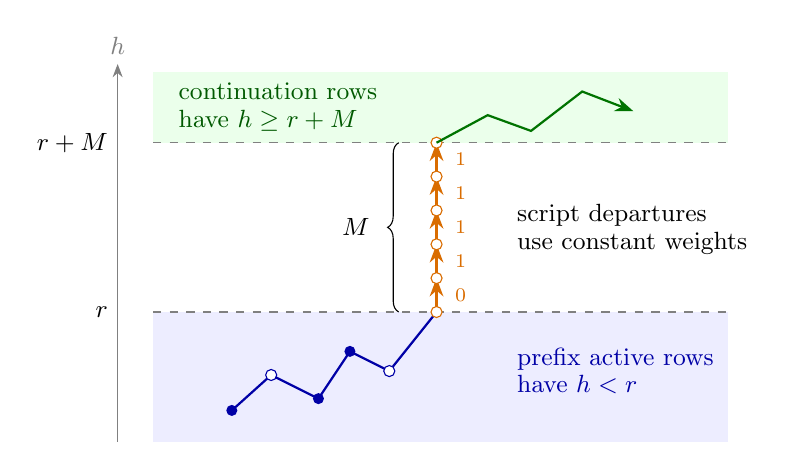
\begin{tikzpicture}[x=1cm,y=1cm,>=Stealth,font=\small]
 \fill[blue!7] (-3.6,-1.65) rectangle (3.7,0);
 \fill[green!8] (-3.6,2.15) rectangle (3.7,3.05);
 \draw[dashed,gray] (-3.6,0)--(3.7,0);
 \draw[dashed,gray] (-3.6,2.15)--(3.7,2.15);
 \draw[->,gray] (-4.05,-1.65)--(-4.05,3.15) node[above] {$h$};
 \node[left] at (-4.05,0) {$r$};
 \node[left] at (-4.05,2.15) {$r+M$};
 \draw[thick,blue!65!black]
   (-2.6,-1.25)--(-2.1,-.8)--(-1.5,-1.1)--(-1.1,-.5)
   --(-.6,-.75)--(0,0);
 \foreach \x/\y in {-2.6/-1.25,-1.5/-1.1,-1.1/-.5}
   \fill[blue!65!black] (\x,\y) circle (2pt);
 \foreach \x/\y in {-2.1/-.8,-.6/-.75}
   \draw[blue!65!black,fill=white] (\x,\y) circle (2pt);
 \foreach \y/\yy/\m in {0/.43/0,.43/.86/1,.86/1.29/1,1.29/1.72/1,1.72/2.15/1}
   \draw[->,thick,orange!85!black] (0,\y)--(0,\yy)
      node[midway,right=3pt] {\scriptsize $\m$};
 \foreach \y in {0,.43,.86,1.29,1.72,2.15}
   \draw[orange!85!black,fill=white] (0,\y) circle (2pt);
 \draw[thick,green!45!black,->]
   (0,2.15)--(.65,2.5)--(1.2,2.3)--(1.85,2.8)--(2.5,2.55);
 \node[align=left,anchor=west,blue!65!black] at (.9,-.75)
   {prefix active rows\\[-1pt]have $h<r$};
 \node[align=left,anchor=west,green!35!black] at (-3.4,2.6)
   {continuation rows\\[-1pt]have $h\ge r+M$};
 \node[align=left,anchor=west] at (.9,1.05)
   {script departures\\[-1pt]use constant weights};
 \draw[decorate,decoration={brace,amplitude=4pt}]
   (-.48,0)--(-.48,2.15) node[midway,left=7pt] {$M$};
\end{tikzpicture}
\caption{The gap at a candidate, shown schematically in height
coordinates.  Filled points indicate active prefix departures; orange
arrows are the constant-weight script steps.  The height gap
separates every active prefix row from every permitted continuation row
by more than \(R\) in \(\ell^\infty\)-distance, although the script
itself visits the intervening sites.}
\label{fig:cut-gap}
\end{figure}

Consequently, conditional on any finite marked prefix ending at a
record, the probability that the script occurs next and ends at a cut
is exactly
\begin{equation}\label{eq:script-probability}
 \xi p_v.
\end{equation}
More precisely, if \(\gamma_0\) is that prefix and \(B\) is any
event for a translated continuation from zero, then
\begin{equation}\label{eq:record-suffix-factorization}
 \begin{split}
 &P_0\{\text{prefix }\gamma_0,\ \text{then the script,}\\
 &\hspace{12mm}\text{then a translated continuation in }B\cap D_v\}\\
 &\hspace{12mm}=W(\gamma_0)\xi P_0(B\cap D_v).
 \end{split}
\end{equation}
Here and below a translated continuation records its positions
relative to its own starting site.  Lemma~\ref{lem:separated-weights}
proves this identity, using the forbidden halfspace below the script's
endpoint and stationarity.

We also record an elementary consequence of ellipticity that will be
used repeatedly.  A walk started in a slab
\(\{x:a\le h(x)\le b\}\), with \(a,b\) finite, exits that slab
almost surely under every uniformly elliptic quenched law.  Choose an
integer \(m>b-a\).  From any site of the slab, \(m\) consecutive
steps \(a_v\) leave it, and their probability is at least
\(\kappa^m\).  Conditional trials in successive blocks of \(m\)
steps bound the probability of remaining for \(jm\) steps by
\((1-\kappa^m)^j\).  In particular, on \(D_v\) the height supremum
is almost surely infinite: remaining forever in \([0,b]\) is null for
each positive integer \(b\).

To describe the pieces between cuts, call a finite marked word
\(\gamma\) from zero a \emph{regeneration word} if it has the
following properties:
\begin{enumerate}[label=(\roman*),leftmargin=*]
 \item all its heights are nonnegative;
 \item it ends at a candidate;
 \item every earlier candidate in the word is undercut later within
       the word, meaning that a subsequent height is strictly smaller
       than that candidate's height.
\end{enumerate}
Records and candidates in this definition are computed within the
word.  Its \emph{width} \(L(\gamma)\) is its terminal height.  The
last script starts at a record of height \(L(\gamma)-M\), so
\begin{equation}\label{eq:word-height-support}
 \begin{gathered}
 L(\gamma)\ge M,\qquad
 0\le h(x)<L(\gamma)\quad(x\in\Dep(\gamma)),\\
 h(x)<L(\gamma)-M\quad(x\in\operatorname{Act}(\gamma)).
 \end{gathered}
\end{equation}
We sometimes call a regeneration word a \emph{slab}, referring to this
height support.

\begin{proposition}[Regeneration law]\label{prop:cut-law}
Fix a normalized real direction \(v\) and suppose \(p_v>0\).
\begin{enumerate}[label=(\roman*),leftmargin=*]
 \item Under the raw law \(P_0\), on
       \(\{\sup_n h(X_n)=\infty\}\) there is a cut almost surely.
 \item Under \(\widehat P_v\), there are infinitely many cuts.  With
       time zero counted as an initial boundary, the relative marked
       words between successive boundaries are independent and
       identically distributed.  Their common law \(\nu_v\) assigns
       mass
       \begin{equation}\label{eq:regeneration-word-law}
        \nu_v(\{\gamma\})=W(\gamma)
       \end{equation}
       to each regeneration word \(\gamma\).  These finite words
       concatenate to the entire conditioned walk.
 \item Under the raw law, conditional on any realized prefix through
       the first cut, the translated suffix has law
       \(\widehat P_v\).  This assertion is restricted to the event
       that a cut exists.
\end{enumerate}
\end{proposition}

\begin{proof}
First test for a scripted cut from time zero.  Failure is detected in
finite time: either the next \(M\) steps are not the script, or they
are the script and the subsequent path first falls below its endpoint.
After a detected failure, wait for a strict record above the whole
maximum attained by the detection time, and test again.  The successive
test starts, when finite, are stopping times in the marked path
filtration.  Equation~\eqref{eq:script-probability}, applied to every
finite record prefix, gives conditional success probability
\(\xi p_v\) at each test.  Hence
\[
 P_0\{\text{the first }j\text{ tests occur and all fail}\}
 \le (1-\xi p_v)^j.
\]
On infinite height supremum, every detected failure is followed by
another finite test start.  Letting \(j\) tend to infinity proves (i).
The slab-exit observation implies that the first cut is finite almost
surely under \(\widehat P_v\).  The tests need not locate the earliest
cut; their only role is to establish that some cut exists.

We now identify the law at the actual first cut by finite prefixes.
Suppose \(\gamma\) is a
regeneration word ending at \(z\).  A path beginning with \(\gamma\)
whose suffix stays at or above \(h(z)\) has its first cut at that
endpoint: all earlier candidates have already been undercut.  It also
satisfies the original \(D_v\).  Conversely, a path in \(D_v\)
through its first cut gives such a word.  Indeed, every earlier
candidate has smaller height than the terminal strict record.  If it
were not undercut before the terminal record, it could not be undercut
afterwards either, since the suffix stays above that record; it would
already be a cut.

For any measurable suffix event \(B\), the row separation in
\eqref{eq:word-height-support} and
Lemma~\ref{lem:separated-weights} therefore give
\[
 \begin{split}
 &P_0\{\text{first-cut prefix }\gamma,\
          \text{ translated suffix in }B\}\\
 &\hspace{25mm}=W(\gamma)P_0(B\cap D_v).
 \end{split}
\]
Dividing by \(p_v\) proves that, under \(\widehat P_v\), the
first word has mass \(W(\gamma)\) and its translated suffix has law
\(\widehat P_v\), independently of that word.  There are only
countably many finite marked words, and the first cut is finite almost
surely, so these masses sum to one.

The cut is a strict record, hence records of its translated suffix are
also records of the full path.  A script cannot straddle this boundary:
such a script would overlap the script that has just ended.  Thus the
cuts of the suffix are precisely the subsequent cuts of the full path.
Iterating the preceding factorization proves the iid assertion in
(ii).  Every word is finite and contains at least \(M\) steps, so the
successive cut times tend to infinity and the words cover the whole
path.

For (iii), the prefix through the raw first cut may have negative
heights, but it still ends with the script from a record, and
every preceding candidate is undercut within the prefix.  Its active
departures lie strictly below the start of the terminal script.  The
same separated-weight calculation gives raw prefix probability
\(W(\gamma)p_v\) and, with suffix restriction \(B\), probability
\(W(\gamma)P_0(B\cap D_v)\).  Their ratio is
\(\widehat P_v(B)\).  All of these arguments enumerate finite
prefixes; none uses a Markov property at a cut selected using the
future.
\end{proof}

\subsection{Escape signs and finite mean width}

The regeneration law gives two consequences needed in the remainder of
the proof.  First, a positive escape probability in one direction rules
out oscillation between arbitrarily high and low levels.  Second, the
widths of the regeneration words have finite mean.  Counting records,
rather than integer height levels, will give the latter conclusion for
real directions as well.

\begin{proposition}[Directional sign union]\label{prop:sign-union}
For every fixed \(v\ne0\),
\begin{equation}\label{eq:sign-union}
 P_0(A_v)>0\quad\Longrightarrow\quad
 p_v>0\ \text{ and }\ P_0(A_v\cup A_{-v})=1.
\end{equation}
More precisely, when \(p_v>0\), infinite height supremum implies
\(A_v\) almost surely, and finite height supremum implies \(A_{-v}\)
almost surely.
\end{proposition}

\begin{proof}
Assume first that \(p_v>0\).  On infinite supremum there is a first
cut, and its suffix has the iid word law of
Proposition~\ref{prop:cut-law}.  The successive slab bases increase in
height by at least \(M\); within each slab the path stays above its
base.  Since each slab is finite, \(h(X_n)\to+\infty\).

For finite supremum, fix integers \(m,b\ge0\).  Consider the event
that all heights are at most \(m\), but heights at least \(-b\) are
visited infinitely often.  From each such visit, a script of
\(m+b+1\) consecutive steps \(a_v\), with no mark restriction,
crosses \(m\) with conditional probability at least
\(\kappa^{m+b+1}\).  Take successive visit trials at least
\(m+b+1\) times apart.  The probability that the first \(j\) trials
occur and all fail to cross \(m\) is at most
\((1-\kappa^{m+b+1})^j\).  The event in question is therefore null.
Taking the countable union over \(m,b\) shows that finite supremum
forces \(h(X_n)\to-\infty\).

It remains to obtain \(p_v>0\) from a positive probability of
\(A_v\).  On \(A_v\), the height sequence tends to infinity, so its
global minimum is attained at some finite time, even if its possible
values are not discrete.  Thus for some deterministic \(n\ge0\)
and \(x\in\ZZ^d\), the event
\[
 \{X_n=x,\ h(X_{n+j})\ge h(x)\text{ for all }j\ge0\}
\]
has positive annealed probability.  If \(q_x(\omega)\) denotes the
quenched probability from \(x\) of staying above \(h(x)\), the
quenched Markov property at time \(n\) expresses this probability as
\(E_Q[P_{0,\omega}(X_n=x)q_x(\omega)]\).  It is bounded above by
\(E_Qq_x=p_v\), by stationarity.  Therefore \(p_v>0\), and the
two alternatives just proved give \eqref{eq:sign-union}.
\end{proof}

\begin{proposition}[Finite mean spatial width]\label{prop:mean-width}
For every normalized real direction \(v\) with \(p_v>0\), the
regeneration law of Proposition~\ref{prop:cut-law} satisfies
\begin{equation}\label{eq:finite-mean-width}
 E_{\nu_v}L<\infty.
\end{equation}
\end{proposition}

\begin{proof}
Let \(S(\gamma)\) be the number of ordinary records in a regeneration
word \(\gamma\), excluding its initial boundary and including its
terminal record.  Each increase of the running maximum is at most one,
because every step has height increment at most one.  Therefore
\(L(\gamma)\le S(\gamma)\).  The record indices of successive cuts,
with index zero at the initial boundary, are sums of iid positive
integer increments with law \(S\): the terminal height of each word
is the maximum so far, so record counts concatenate across boundaries.

For \(i\ge0\), let \(\rho_i\) be the time of ordinary record
index \(i\) in a raw walk, with \(\rho_0=0\) and
\(\rho_i=\infty\) if that record is never reached.  Put
\[
 D'_{v,i}=\{\rho_i<\infty,\ h(X_j)\ge0
                       \text{ for }0\le j\le\rho_i\}.
\]
A script from record \(i\) creates exactly \(M\) consecutive
strict records.  Hence a cut of record index \(i+M\), on a path in
\(D_v\), occurs exactly when the prefix realizes \(D'_{v,i}\),
the script follows, and its suffix stays above its endpoint.  Summing
\eqref{eq:record-suffix-factorization} over the possible record
prefixes and dividing by \(p_v\) gives
\begin{equation}\label{eq:record-renewal-lower}
 \widehat P_v\{i+M\text{ is a cut index}\}
   =\xi P_0(D'_{v,i})\ge\xi p_v.
\end{equation}
The inequality holds because on \(D_v\) the supremum is infinite
almost surely, so every ordinary record is reached.

Let \(N_{\mathrm{rec}}(n)\) count the cut indices in \(\{1,\ldots,n\}\).
Equation~\eqref{eq:record-renewal-lower} implies
\[
 \liminf_{n\to\infty}
 \frac{E_{\widehat P_v}N_{\mathrm{rec}}(n)}{n}\ge\xi p_v>0.
\]
If \(E_{\nu_v}S=\infty\), however, the partial sums of iid copies
of \(S\), divided by their number, tend to infinity almost surely.
To see this, apply the strong law to \(\min(S,K)\) for each positive
integer \(K\), then let \(K\to\infty\).  Inverting these partial
sums shows \(N_{\mathrm{rec}}(n)/n\to0\) almost surely.  Since this
ratio lies in \([0,1]\), bounded convergence gives the same limit in
expectation, a contradiction.  Thus \(E_{\nu_v}S<\infty\), and
\(L\le S\) proves \eqref{eq:finite-mean-width}.
\end{proof}

The estimate concerns spatial width; it uses no moment assumption on
the time spent in a word.  We next show that coexistence of the two
escape signs also forces a finite mean for the full spatial radius.

\section{Spatial moments and reduction to a coordinate direction}
\label{sec:radius}

The finite mean width from Proposition~\ref{prop:mean-width} controls a
regeneration word only in its direction of progress.  We now show that
coexistence of the two escape signs also controls its spatial extent.
This will give two limiting rays and reduce the problem to a coordinate
direction.  The radius argument adapts
\cite[Proposition~3.1]{OpenAI2026}, with a marked connector and a
separated infinite continuation supplying the finite-range version.

For a regeneration word $\gamma$ with position sequence
$(x_0,\ldots,x_m)$, written relative to $x_0=0$, define its radius by
\[
  \mathcal R(\gamma)=\max_{0\le j\le m}|x_j|,
\]
where $|\cdot|$ denotes Euclidean norm.  In particular, the terminal
arrival contributes to the radius.  Distances used for finite-range
independence remain $\ell^\infty$ distances.

\subsection{An integrable spatial radius}

We first record an elementary estimate that controls all initial sums at
once.  Stationarity, rather than independence, is enough for this estimate.
It is the stationary-sequence form of Hopf's maximal ergodic inequality;
see Garsia~\cite{Garsia1965}.  We include a disjoint-interval proof.

\begin{lemma}[A maximal estimate for initial averages]
\label{lem:stationary-maximal}
Let $(Z_i)_{i\ge1}$ be a stationary sequence of nonnegative integrable
random variables.  For every integer $n\ge1$ and every $a>0$,
\[
  \PP\left\{\max_{1\le k\le n}\frac1k\sum_{i=1}^k Z_i>a\right\}
  \le \frac{\EE Z_1}{a}.
\]
\end{lemma}

\begin{proof}
Call an integer $j\ge1$ bad if some interval starting at $j$, of length
at most $n$, has average greater than $a$.  Among the bad starts in
$\{1,\ldots,m\}$, select the leftmost one and a witnessing interval.
Continue by selecting the leftmost bad start strictly to the right of
the selected interval, and repeat.  These disjoint intervals cover all
bad starts in $\{1,\ldots,m\}$ and lie in $\{1,\ldots,m+n\}$.
Their total length is at least the number of those bad starts, while
the sum of the $Z_i$ over them is at least $a$ times their total length.
Consequently
\[
  a\,\#\{j\le m:j\text{ is bad}\}\le\sum_{i=1}^{m+n}Z_i.
\]
Taking expectations, using stationarity, dividing by $m$, and letting
$m\to\infty$ proves the assertion.
\end{proof}

\begin{proposition}[Radius moment under coexistence]
\label{prop:radius-moment}
Let $v\ne0$ satisfy $\|v\|_\infty=1$.  If
$P_0(A_v)>0$ and $P_0(A_{-v})>0$, then the regeneration-word laws of
Proposition~\ref{prop:cut-law} satisfy
\begin{equation}
  E_{\nu_v}\mathcal R+E_{\nu_{-v}}\mathcal R<\infty.
  \label{eq:radius-moment}
\end{equation}
\end{proposition}

\begin{proof}
Both nonbacktracking probabilities $p_v,p_{-v}$ are positive by
Proposition~\ref{prop:sign-union}.  For $\sigma\in\{+,-\}$ write
\[
  P_\sigma^*=\widehat P_{\sigma v},\qquad
  E_\sigma^*=E_{P_\sigma^*}.
\]
Here $\sigma v$ means $v$ or $-v$, respectively.  Under either law, let
$L_i,\mathcal R_i$ be the width and radius of its $i$th regeneration
word, and put
\[
  H_0=0,\qquad H_k=\sum_{i=1}^k L_i.
\]
An unsubscripted $L$ or $\mathcal R$ denotes the corresponding variable
for one word.  All constants chosen below are independent of the scale
parameters $i_0$ and $a$.

Suppose that \eqref{eq:radius-moment} fails.  The truncated mean
\[
  I(t)=\sum_{\sigma\in\{+,-\}}E_\sigma^*\min(\mathcal R,t),
  \qquad t\ge0,
\]
is then nondecreasing and unbounded.  It is concave, $I(0)=0$, and
$I(t)=o(t)$: the last assertion follows by dominated convergence from
the almost-sure finiteness of each regeneration word.

We will obtain a fixed positive probability that the final supremum of
one of the two signed heights lies in a bounded window, and then place
these windows arbitrarily far apart.  The unbounded truncated mean
will produce a large spatial excursion after a controlled initial
segment, and hence a record for a tilted linear functional.  A marked
connector will let us append a separated continuation in the opposite
direction while preserving the height maximum already attained.

\paragraph{The scale and a controlled initial segment.}
Proposition~\ref{prop:mean-width} and the strong law allow us to choose
$c,C>0$ and $C_0\ge0$ so that, under each sign law, with probability
greater than $0.95$,
\begin{equation}
  ck-C_0\le H_k\le Ck+C_0\qquad(k\ge0).
  \label{eq:radius-height-bounds}
\end{equation}
Indeed, choose $c$ below both mean widths and $C$ above both, and then
choose a deterministic $C_0$ controlling the finitely many initial
deviations with the stated probability.  Next choose an integer
$C_1\ge1$, a number $b>1/c$, a number $B>1$, and $\eta>0$, in that
order, with
\begin{equation}
  C_1c>C+4,\qquad
  \frac{B-1}{\sqrt d}-b(C+2)>2,\qquad
  4C_1\eta<0.15.
  \label{eq:radius-constants}
\end{equation}

For $a>0$ sufficiently large, let $N=N(a)$ be the first positive integer
such that
\[
  I(aN)\ge\eta a.
\]
It exists because $I$ is unbounded, and $N(a)\to\infty$ because
$I(t)=o(t)$.  For large $a$, minimality and concavity give
\begin{equation}
  \eta a\le I(aN)
  \le\frac{N}{N-1}I(a(N-1))<2\eta a.
  \label{eq:radius-scale}
\end{equation}

Let $\mathcal J_m$ be the event that
\eqref{eq:radius-height-bounds} holds through $m$ and
\[
  \sum_{i=1}^k\mathcal R_i\le ak\qquad(1\le k\le m).
\]
For both signs and all sufficiently large $a$,
\begin{equation}
  P_\sigma^*(\mathcal J_{C_1N})>0.8.
  \label{eq:radius-controlled}
\end{equation}
To see this, set $n=C_1N$ and truncate each radius at $an$.
Its mean is at most
\[
  I(an)\le C_1 I(aN)<2C_1\eta a.
\]
Lemma~\ref{lem:stationary-maximal} bounds by $2C_1\eta$ the probability
that any initial average of the truncated radii, through $n$, exceeds
$a$.  Also
\[
  P_\sigma^*\{\mathcal R_i>an\text{ for some }i\le n\}
  \le nP_\sigma^*(\mathcal R>an)
  \le\frac{E_\sigma^*\min(\mathcal R,an)}a
  <2C_1\eta.
\]
Combining these estimates with the probability of
\eqref{eq:radius-height-bounds} proves
\eqref{eq:radius-controlled}.

\paragraph{A large excursion following that segment.}
Choose an integer $i_0$ large enough that
\begin{equation}
\begin{gathered}
  \sum_\sigma\sum_{i\ge i_0}P_\sigma^*(L>i)<\frac{\eta}{4B},\\
  c(i-1)-C_0\ge\frac{ci}{2},\qquad
  C(i-1)+C_0+i\le(C+2)i\qquad(i\ge i_0).
\end{gathered}
\label{eq:radius-initial-index}
\end{equation}
The first condition follows from integrability of the widths.
With $i_0$ fixed, take $a$ sufficiently large that $N\ge i_0$ and
$I(Bai_0)<\eta a/4$, as well as all preceding large-$a$ requirements.
For $i_0\le i\le N$ define
\[
  \mathcal L_i=\{\mathcal R_i>Bai,\ L_i\le i\},\qquad
  \Lambda_\sigma=\sum_{i=i_0}^N P_\sigma^*(\mathcal L_i).
\]
Integration of the decreasing radius tails gives
\begin{align*}
  \sum_\sigma\sum_{i=i_0}^N P_\sigma^*(\mathcal R>Bai)
  &\ge\frac{I(Ba(N+1))-I(Bai_0)}{Ba},\\
  \sum_\sigma\sum_{i=1}^N P_\sigma^*(\mathcal R>Bai)
  &\le\frac{I(BaN)}{Ba}.
\end{align*}
The first right-hand side is at least $3\eta/(4B)$, by
\eqref{eq:radius-scale} and monotonicity of $I$.  The second is at most
$2\eta$, by concavity.  Subtracting the width-tail bound in
\eqref{eq:radius-initial-index} therefore yields
\begin{equation}
  \frac{\eta}{2B}\le\Lambda_++\Lambda_-\le2\eta.
  \label{eq:radius-large-excursion-mass}
\end{equation}

Choose a sign $\sigma$ for which $\Lambda_\sigma\ge\eta/(4B)$, and count
the indices for which both $\mathcal J_{i-1}$ and $\mathcal L_i$ occur.
Independence of the $i$th word from its predecessors and
\eqref{eq:radius-controlled} give a mean of at least
$0.8\Lambda_\sigma$.  The second moment is at most
$\Lambda_\sigma+\Lambda_\sigma^2$, by domination by the sum of the
independent indicators $\one_{\mathcal L_i}$.
Cauchy--Schwarz and \eqref{eq:radius-large-excursion-mass} imply that,
with probability at least a constant $\delta>0$ independent of $i_0,a$,
there is an index $i\in[i_0,N]$ with
\begin{equation}
  \mathcal J_{i-1}\cap\mathcal L_i.
  \label{eq:radius-selected-excursion}
\end{equation}

\paragraph{A record in a tilted direction.}
For this sign write $h(x)=\sigma v\cdot x$.  On
\eqref{eq:radius-selected-excursion}, all preceding positions have norm
at most $a(i-1)$, whereas some position $X$ in word $i$ satisfies
$|X|>(B-1)ai$.  Hence, for some coordinate step $u\in U$,
\[
  u\cdot X>\frac{(B-1)ai}{\sqrt d}.
\]
Throughout this word, the running maximum of $h$ lies between
$H_{i-1}$ and $H_i$, and therefore in
$[ci/2,(C+2)i]$.  Define the linear functional
\[
  Y(x)=u\cdot x-ba h(x).
\]
Before word $i$, nonnegativity of $h$ gives $Y\le a(i-1)$.
At the indicated position, \eqref{eq:radius-constants} gives $Y>2ai$.
There is consequently a strict $Y$-record whose running $h$-maximum
belongs to the deterministic window
\begin{equation}
  \mathcal W=[ci_0/2,(C+2)N].
  \label{eq:radius-window}
\end{equation}

For each fixed $u$, let $T$ be the first positive time at which the
position is a strict $Y$-record, the running $h$-maximum belongs to
$\mathcal W$, and the entire prefix has nonnegative $h$-heights.
These conditions make $T$ a stopping time.  Since there are $2d$
choices of $u$, one of them satisfies
$P_\sigma^*(T<\infty)\ge\delta/(2d)$.  Fix that choice and set
$p_* = \min(p_v,p_{-v})$.  Under the raw law,
\begin{equation}
  P_0(T<\infty)\ge\frac{p_*\delta}{2d}.
  \label{eq:radius-record-probability}
\end{equation}

We have found a record with a uniformly positive probability, while its
running height maximum lies in a window that can be moved arbitrarily
far out.  We next continue from this record so that the final height
maximum stays in the same window.  The continuation must remain
separated from the observed prefix for its annealed probability to
factor.

\paragraph{A separated continuation in the opposite direction.}
Choose a coordinate step $e$ with $h(e)=-1$.  From $X_T$ force $m_0$
successive steps $e$, all with mark $0$, where $m_0$ is a fixed positive
integer satisfying
\begin{equation}
  m_0b>1+bC_0+Rdb+1.
  \label{eq:radius-connector-length}
\end{equation}
The choice of $m_0$ depends only on the fixed constants $b,C_0,R,d$,
and is independent of $i_0,a$.
These steps have weight $\lambda^{m_0}$.  At their endpoint
$z=X_T+m_0e$, consider the translated raw event consisting of
$D_{-\sigma v}$ and $\mathcal J_{C_1N}$ for the opposite regeneration
sequence, with the required cuts finite.  Its raw probability is at
least $0.8p_*$ by \eqref{eq:radius-controlled} and
Proposition~\ref{prop:cut-law}.

Every position of the continuation from $z$ is separated by more than
$R$ from the prefix through $T$.  There are two parts to this geometric
assertion.
During opposite word $k+1$, for $0\le k<C_1N$, displacement from $z$
in the $u$ coordinate is at least $-a(k+1)$, by the initial-sum radius
bound in $\mathcal J_{C_1N}$; displacement in $h$ is at most $-ck+C_0$.
Its total $Y$-increment from $X_T$, including
the forced steps, is therefore at least
\begin{align}
  &m_0(ba-1)-a(k+1)+ba(ck-C_0)\notag\\
  &\hspace{12mm}
  =a\bigl(m_0b-1-bC_0+(bc-1)k\bigr)-m_0.
  \label{eq:radius-tilted-gap}
\end{align}
Since $bc>1$, \eqref{eq:radius-connector-length} makes this quantity
greater than $R(1+dba)$ for all sufficiently large $a$, uniformly in
$k$.  Every prefix position has $Y$-value at most $Y(X_T)$, while
\[
  |Y(x)-Y(y)|\le(1+dba)\|x-y\|_\infty.
\]
Thus the first $C_1N$ opposite words are at distance greater than $R$
from every prefix position.

At the end of these words the absolute $h$-coordinate is at most
\begin{equation}
  (C+2)N-m_0-cC_1N+C_0<-dR
  \label{eq:radius-tail-gap}
\end{equation}
for large $a$, by \eqref{eq:radius-constants}.  All subsequent positions
stay at or below this height, since this endpoint is a cut in direction
$-\sigma v$.  The prefix has nonnegative $h$-heights and
$|h(x)-h(y)|\le d\|x-y\|_\infty$, so the entire remaining tail is
also separated from the prefix.  The tilted inequality protects the
initial opposite words; the height inequality protects everything
after their last cut.  No bound on $Y$ is required for this remaining tail.

We now justify the probability calculation for this infinite
continuation.  Fix a finite marked prefix $\gamma$ realizing $T$, and
let $A_\gamma$ be its set of positions, including its terminal arrival.
The preceding deterministic bounds show that every path in the
specified continuation event avoids the closed $R$-neighborhood of
$A_\gamma$.  Consequently its quenched probability can be computed
using the walk killed on first arrival in that neighborhood.  By
Lemma~\ref{lem:separated-weights}, this probability depends only on
rows outside the neighborhood, even though the event specifies future
cuts and an infinite nonbacktracking tail.  Those rows are separated
from the active departures of $\gamma$.

The forced connector has constant quenched weight and reveals no rows.
The weight of $\gamma$, the connector, and the continuation therefore
factors as
\[
  W(\gamma)\lambda^{m_0}
  P_0\{D_{-\sigma v},\ \mathcal J_{C_1N}
                 \text{ for its regeneration sequence}\}
  \ge 0.8p_*\lambda^{m_0}W(\gamma).
\]
Here stationarity identifies the last factor with the raw probability
from $z$, and the almost-sure existence of the indicated cuts under
$D_{-\sigma v}$ is understood.  This use of separated rows is made
after fixing $\gamma$; no independence for a randomly chosen region is
assumed.

The connector decreases $h$, and the opposite continuation stays at
or below its own initial height.  Thus the final supremum of $h$ is
exactly the running supremum at $T$ and belongs to $\mathcal W$.
Summing over the disjoint prefixes realizing $T$ and using
\eqref{eq:radius-record-probability} yields
\begin{equation}
  P_0\left\{\sup_{n\ge0}\sigma v\cdot X_n\in\mathcal W\right\}
  \ge\rho,
  \qquad
  \rho:=\frac{0.8\lambda^{m_0}p_*^2\delta}{2d}>0.
  \label{eq:radius-final-supremum}
\end{equation}

Finally, choose $i_0$ and then $a$ successively so that the resulting
windows \eqref{eq:radius-window} are pairwise disjoint.  This is
possible by taking each new lower endpoint beyond the preceding upper
endpoint before choosing its $a$.  The sign $\sigma$ may change from
one window to the next, but for either fixed sign the corresponding
final-supremum events are disjoint.  Their probabilities, summed over
all windows and both signs, are at most $2$, contradicting the uniform
lower bound \eqref{eq:radius-final-supremum}.  This proves
\eqref{eq:radius-moment}.
\end{proof}

\subsection{Opposite limiting rays}

The radius moment controls the path between cuts, so the ordinary
strong law for regeneration displacements also describes the full
trajectory.  The limiting-ray argument and the coordinate reduction
follow \cite[Section~4.1]{OpenAI2026}.

\begin{lemma}[Limiting rays under coexistence]
\label{lem:opposite-rays}
Under the coexistence hypotheses of Proposition~\ref{prop:radius-moment},
there are deterministic unit vectors $r_+,r_-$ such that, for
$\sigma\in\{+,-\}$,
\[
  |X_n|\longrightarrow\infty,\qquad
  \frac{X_n}{|X_n|}\longrightarrow r_\sigma
  \quad P_0\text{-almost surely on }A_{\sigma v}.
\]
They satisfy $r_\sigma\cdot(\sigma v)>0$ and $r_-=-r_+$.
\end{lemma}

\begin{proof}
The terminal displacement of a word of law $\nu_{\sigma v}$ is
integrable by Proposition~\ref{prop:radius-moment}.  Write its mean as
$b_\sigma'\in\RR^d$.  Since
\[
  b_\sigma'\cdot(\sigma v)=E_{\nu_{\sigma v}}L>0,
\]
this vector is nonzero.  Under $\widehat P_{\sigma v}$, the $k$th cut
location divided by $k$ tends almost surely to $b_\sigma'$.
Integrability also gives $\mathcal R_k/k\to0$ almost surely: for each
$\varepsilon>0$, the sum of
$\widehat P_{\sigma v}(\mathcal R_k>\varepsilon k)$ is finite, and
Borel--Cantelli applies.  Between consecutive cuts the displacement
from the earlier cut is bounded by the next radius.  Since the number
of completed words tends to infinity along the trajectory, it follows
that $|X_n|\to\infty$ and
\[
  \frac{X_n}{|X_n|}\longrightarrow
  r_\sigma:=\frac{b_\sigma'}{|b_\sigma'|}.
\]
Under the raw law on $A_{\sigma v}$, the first cut is finite and its
translated suffix has law $\widehat P_{\sigma v}$ by
Proposition~\ref{prop:cut-law}; hence the same conclusion holds there.

The signs of the projections on $v$ make $r_+$ and $r_-$ distinct.
Suppose they are not opposite.  Then $w=r_++r_-$ is nonzero and
\[
  w\cdot r_+=w\cdot r_-=1+r_+\cdot r_->0.
\]
Proposition~\ref{prop:sign-union} gives
$P_0(A_v\cup A_{-v})=1$, so the limiting rays imply $P_0(A_w)=1$.
Rescale $w$ to have $\ell^\infty$ norm one and apply the cut
construction in that direction.

Under $\widehat P_w$, the limiting ray exists almost surely because
this law is a conditioning of the raw law just considered.  Its value
is unchanged on deleting any finite number of regeneration words and
translating the remaining path: such operations do not affect a
limiting direction when positions tend to infinity in norm.
Consequently it is a tail random variable of the iid words under
$\widehat P_w$: for every $k$, its value can be computed from the words
after $k$.  The independent tail zero--one law makes it
deterministic.  Since $P_0(A_w)=1$, the raw walk has a first cut in
direction $w$ almost surely, with translated suffix law
$\widehat P_w$.  Its limiting ray must therefore have that same
deterministic value almost surely.  This contradicts the two distinct
rays $r_+,r_-$, each occurring with positive raw probability.  Hence
$r_-=-r_+$.
\end{proof}

\begin{proposition}[Reduction to a coordinate direction]
\label{prop:coordinate-reduction}
If $0<P_0(A_v)<1$ for some fixed nonzero real direction $v$, then there
is a coordinate $i\in\{1,\ldots,d\}$ such that
\[
  P_0(A_{e_i})>0\qquad\text{and}\qquad P_0(A_{-e_i})>0.
\]
\end{proposition}

\begin{proof}
After normalizing $v$, Proposition~\ref{prop:sign-union} shows that
both signs of escape in direction $v$ have positive probability.
Choose a coordinate with nonzero projection on the opposite rays
from Lemma~\ref{lem:opposite-rays}.  Along one ray this coordinate
tends to $+\infty$, and along the other it tends to $-\infty$.
Each ray occurs with positive probability, giving the assertion.
\end{proof}

To prove Theorem~\ref{thm:main}, it therefore remains to exclude
coexistence in a coordinate direction.  After permuting coordinates,
we may take that direction to be $e_1$.

\section{Coordinate bridges and opposed paths}
\label{sec:bridges}

By Proposition~\ref{prop:coordinate-reduction}, it remains to exclude
coexistence in a coordinate direction. We therefore assume for the rest of
the proof that both $A_{e_1}$ and $A_{-e_1}$ have positive probability.
The two corresponding slab laws have finite mean width and finite mean
radius, by Propositions~\ref{prop:mean-width} and
\ref{prop:radius-moment}. We will arrange independent sequences of these
slabs in opposite chronological directions. The contradiction will come
from two estimates on how often the resulting paths approach each other.
The bridge and opposed-path constructions follow the corresponding iid
strategy in \cite[Sections~4.2--4.3]{OpenAI2026}. We give their marked
versions here, including the separation arguments for the present
environment law.

For $\sigma\in\{+,-\}$, with $\sigma e_1$ denoting $e_1$ or $-e_1$, write
\[
 \widehat P_\sigma=\widehat P_{\sigma e_1},\qquad
 D_\sigma=D_{\sigma e_1},\qquad p_\sigma=p_{\sigma e_1}>0,
 \qquad \nu_\sigma=\nu_{\sigma e_1}.
\]
For a walk starting at the origin, let $T_j^\sigma$ be the first hit of
signed coordinate height $\sigma x_1=j$. For integers $n\ge0$, set
\begin{equation}
 u_n^\sigma=P_0(T_n^\sigma<T_{-1}^\sigma),
 \qquad F_\sigma(n)=\nu_\sigma(L>n).
 \label{eq:hitting-width-tail}
\end{equation}
Thus $u_0^\sigma=1$, and $u_n^\sigma$ decreases to a limit at least
$p_\sigma$: on $D_\sigma$, the signed height reaches every positive integer
almost surely. Constants below may depend on the fixed environment law,
$d,\kappa,R$, and the chosen script, but not on any of the scale parameters.

\subsection{Bridges ending at prescribed cuts}

Under $\widehat P_\sigma$, the widths of successive slabs form a renewal
process on the nonnegative integers. Let $\bar u_n^\sigma$ be its renewal
mass, including the initial renewal at zero. Equivalently, it is the
probability of a cut at signed height $n$, with the initial boundary counted
as a cut. To identify the corresponding finite path law, for $H\ge M$ let
$\mathcal D_H^\sigma$ be the following event for the raw marked walk: it
first hits $H-M$ before $-1$ in signed height, and from that hit it takes
the prescribed $M$-step script. The script ends at its first hit of $H$.

If $\bar u_H^\sigma>0$, let $\mathcal B_H^\sigma$ denote the law of the slab
list through height $H$, conditional on a cut there. At $H=0$ this law is
concentrated on the empty list. We call $\mathcal B_H^\sigma$ the
\emph{exact-cut bridge law}.

\begin{proposition}[Exact-cut bridges]
\label{prop:exact-cut-bridges}
The renewal masses satisfy
\begin{equation}
 \bar u_0^\sigma=1,\qquad
 \bar u_j^\sigma=0\quad(1\le j<M),\qquad
 \bar u_H^\sigma=\xi u_{H-M}^\sigma\quad(H\ge M).
 \label{eq:bridge-renewal}
\end{equation}
For a list of slabs $(\gamma_1,\ldots,\gamma_m)$ with total width $H$, its
mass under $\mathcal B_H^\sigma$ is
\begin{equation}
 \mathcal B_H^\sigma(\gamma_1,\ldots,\gamma_m)
   =\frac{\prod_{i=1}^m W(\gamma_i)}{\bar u_H^\sigma}.
 \label{eq:bridge-law}
\end{equation}
In particular, reversing the list order preserves this law; the steps
within each word retain their original order.

For $H\ge M$, concatenating the list gives the raw marked path through its
first hit of $H$, conditioned on $\mathcal D_H^\sigma$. Each such path has
a unique parsing into slabs. Concatenating any prescribed slab words, or
successive bridges of prescribed widths, gives a raw path weight equal to
the product of the constituent raw weights.
\end{proposition}

\begin{proof}
The raw probability of $\mathcal D_H^\sigma$ is
$\xi u_{H-M}^\sigma$. Its terminal script begins at a record and ends at
a candidate of height $H$. By the script gap and
Lemma~\ref{lem:separated-weights}, imposing a suffix that stays at signed
height at least $H$ multiplies this probability by $p_\sigma$.
Conversely, a cut at $H$ must be the end of the script beginning at the
first hit of $H-M$: coordinate records are first hits, and each scripted
step increases the signed height by one. Dividing by $p_\sigma$ to
condition on $D_\sigma$ proves \eqref{eq:bridge-renewal}. No cut can have
width less than $M$.

The iid slab law from Proposition~\ref{prop:cut-law} now gives
\eqref{eq:bridge-law}. Its numerator and the constraint on total width are
unchanged when the list is reversed. Alternatively, for each fixed prefix
through $H$ realizing $\mathcal D_H^\sigma$, the cut suffix supplies the
same factor $p_\sigma$. Conditional on the cut at $H$ under
$\widehat P_\sigma$, the prefix therefore has mass
$W(\text{prefix})/\bar u_H^\sigma$. This is exactly its raw conditional
mass given $\mathcal D_H^\sigma$.

The parsing can be recovered from the finite prefix alone. Select the
candidate ends whose heights are not undercut later in the prefix, and
split at those ends. A suffix staying at or above $H$ cannot change this
selection, because $H$ is a strict record height. Between successive
selected candidates, every earlier candidate is undercut, which is
precisely the defining condition for a slab. A script cannot straddle a
selected boundary: it would overlap the script ending there. Thus these
are exactly the slab boundaries, and the parsing is unique.

Finally, active departures of a slab ending at signed height $b$ lie
strictly below $b-M$. All departures of the following slabs lie at or
above $b$. These row sets are more than $R$ apart in infinity distance.
Applying Lemma~\ref{lem:separated-weights} successively, and using
translation invariance, factors the weight of any prescribed
concatenation. The same argument applies after grouping the slabs into
bridges of prescribed widths. Each group boundary is reached on a first
hit, so the grouping introduces no extra path multiplicity.
\end{proof}

The distinction between $u_n^\sigma$ and $\bar u_n^\sigma$ will matter.
The former are ordinary hitting probabilities and decrease with $n$;
the latter have a gap before the first possible script end. The next
estimate retains the contribution of that gap.

\begin{lemma}[Width tails control hitting differences]
\label{lem:width-tail}
For either sign and all integers $n'\ge n\ge0$,
\begin{equation}
 u_n^\sigma-u_{n'}^\sigma
   \le C(n'-n)F_\sigma(n),
 \qquad
 \sum_{l\ge0}2^lF_\sigma(2^l)<\infty.
 \label{eq:width-tail-comparison}
\end{equation}
\end{lemma}

\begin{proof}
Fix a sign and suppress it. Partition according to the last renewal at
or before $m$. The next width exceeds the distance from that renewal to
$m$, so
\[
 \sum_{k=0}^m F(k)\bar u_{m-k}=1.
\]
Subtracting the identity at $m+1$, and using $\bar u_0=1$, gives
\[
 \sum_{k=0}^m F(k)
       (\bar u_{m-k}-\bar u_{m+1-k})=F(m+1).
\]
By \eqref{eq:bridge-renewal}, every adjacent difference in this sum is
nonnegative except the one with $m-k=M-1$, which equals $-\xi$.
Take $m=n+M$. The exceptional index is $k=n+1$, while the term $k=0$
equals $\xi(u_n-u_{n+1})$. Dropping the other nonnegative terms yields
\[
 \xi(u_n-u_{n+1})
   \le F(n+M+1)+\xi F(n+1)
   \le(1+\xi)F(n).
\]
Summation from $n$ to $n'-1$, using that $F$ decreases, proves the first
bound. The second follows by grouping the ordinary tail sum
$\sum_{k\ge0}F(k)=E_{\nu_\sigma}L<\infty$ into dyadic intervals.
\end{proof}

\subsection{Opposed tapes and common blocks}

Take two independent sequences of iid relative slab words, with laws
$\nu_+$ and $\nu_-$. We call these sequences the positive and negative
\emph{tapes}, and denote their joint law and expectation by
$\mathbf P$ and $\mathbf E$. Write
$\pi x=(x_2,\ldots,x_d)$ for the lateral coordinate of $x$.
Place the words in space as follows.
\begin{itemize}[leftmargin=*,itemsep=3pt]
\item The first positive word has its terminal site at $0$. Each
subsequent positive word has its terminal site at the starting site of
the preceding word. Thus tape order moves downward, whereas a finite
initial portion is traversed chronologically by taking its words in
reverse list order, always following the steps of each word forward.
\item The negative words are concatenated in their original order,
starting at $-e_1$. This produces a downward path with law
$\widehat P_-$ translated to $-e_1$.
\end{itemize}
Backward placement of regeneration pieces also appears in Berger's
backward-path construction \cite[Sections~2--3]{Berger2008}.
We measure \emph{depth} by $z=-x_1$. A word of width $L$, preceded by
total width $s$ on its tape, has all its departure depths in
\begin{equation}
                    (s,s+L]\cap\ZZ.
 \label{eq:departure-depths}
\end{equation}
For the positive tape this excludes the terminal arrival at depth $s$.
For the negative tape the same interval results from the initial
one-level offset: its start has depth $s+1$, and its terminal arrival has
depth $s+L+1$.

A \emph{contact} is a positive departure site at infinity distance at
most $R$ from some negative departure site. All departures count,
regardless of their marks. The depth and, subsequently, the block index
of a contact always refer to the positive departure. There is at least
one contact: the last positive departure before its terminal site $0$
is $-e_1$, the initial site of the negative path.

To compare contacts at different depths, we group the two tapes using
their common width renewals. Starting from width zero, end the first
common block at the first positive integer that is a width sum on both
tapes; continue with successive common width sums. The next proposition
shows that this grouping gives iid finite pieces with the spatial
integrability needed below. This is the intersection construction for
independent renewal processes; see \cite{AlexanderBerger2016}.

\begin{proposition}[Common blocks]
\label{prop:common-blocks}
The common blocks exist indefinitely, and their pairs of slab lists are
iid. Their widths $K_i$ have a common law satisfying
\[
                  M\le K_i<\infty\quad\text{a.s.},
             \qquad \mu:=\mathbf E K_i<\infty.
\]
The expected sum of the radii of all slabs on both sides of one common
block is finite. In particular, if
\begin{equation}
 W'_0=0,\qquad W'_i=\sum_{j=1}^iK_j,
 \label{eq:common-width-sums}
\end{equation}
then $W'_i/i\to\mu$ almost surely.
\end{proposition}

\begin{proof}
Let $K$ be the first positive common width, allowing $K=\infty$ for now.
For each fixed pair of finite prefixes that realize $K=k$, the fact
that $k$ is their first common width is decided by those prefixes. Their
unused tails are independent tapes with the initial laws. Enumerating
these prefix pairs therefore gives the renewal recursion
\[
 c_0=1,\qquad
 c_n=\sum_{k=1}^n\mathbf P(K=k)c_{n-k}\quad(n\ge1),
 \qquad c_n=\bar u_n^+\bar u_n^-.
\]
Set $f(t)=\sum_{k\ge1}\mathbf P(K=k)t^k$ for $0<t<1$. Nonnegative
power-series summation gives
\[
 \sum_{n\ge0}c_nt^n=\frac{1}{1-f(t)}.
\]
Equation~\eqref{eq:bridge-renewal} implies
$c_n\ge\xi^2p_+p_->0$ for every $n\ge M$. Hence
$\sum c_nt^n\ge\xi^2p_+p_-t^M/(1-t)$, and consequently
$(1-f(t))/(1-t)$ stays bounded as $t\uparrow1$. First this forces
$f(t)\to1$, proving $K<\infty$ almost surely. We can then write
\[
 \frac{1-f(t)}{1-t}
  =\mathbf E\frac{1-t^K}{1-t}\ \uparrow\ \mathbf E K,
\]
which proves finite mean. The same prefix factorization at each common
renewal proves that the successive pairs of lists are iid. The lower
bound $K\ge M$ follows from the minimum slab width. The strong law gives
the assertion about $W'_i$.

Let $N_+$ be the number of positive words in the first common block.
Since every width is at least one, $N_+\le K$. The event $\{N_+\ge i\}$
is determined by the first $i-1$ positive widths and the entire negative
tape: none of those positive width sums may be a negative width sum.
It is therefore independent of the $i$th positive word and its radius
$\mathcal R_i^+$. Tonelli's theorem gives
\[
 \mathbf E\sum_{i=1}^{N_+}\mathcal R_i^+
  =\sum_{i\ge1}\mathbf P(N_+\ge i)E_{\nu_+}\mathcal R
  =\mathbf E N_+\,E_{\nu_+}\mathcal R<\infty.
\]
The identical argument for the negative tape proves the claimed
integrability, using Proposition~\ref{prop:radius-moment}.
\end{proof}

The notation $W'_i$ records cumulative width and is distinct from the
word weight $W(\gamma)$. By \eqref{eq:departure-depths}, departures in
common block $i$ on either tape have depths in
$(W'_{i-1},W'_i]$. A contact in positive block $i$ can involve a negative
departure only in block $i-1$, $i$, or $i+1$: skipping an entire common
block would give a depth difference greater than $M>R$.

For each common block let $S'_i\in\ZZ^{d-1}$ be the sum of the lateral
displacements of all its positive and negative words, with both
displacements measured in the words' original chronological directions.
The $S'_i$ are iid and
\begin{equation}
                    \mathbf E\abs{S'_i}<\infty.
 \label{eq:lateral-moment}
\end{equation}
Indeed, their norms are bounded by the sums of radii controlled in
Proposition~\ref{prop:common-blocks}. As we pass downward through a
block, the negative anchor moves by its chronological displacement,
whereas the positive anchor moves by the negative of its chronological
displacement. The lateral gap, negative anchor minus positive anchor,
therefore increases by $S'_i$.

We now have both a common block index for the two tapes and integrable
iid increments for their lateral gap. The quantity on which the two
remaining estimates will disagree is
\begin{equation}
 m(J)=\sum_{j=1}^J\mathbf P\bigl\{
  \text{a contact occurs in a positive block of index in }
                      (2^j,2^{j+1}]\bigr\},\qquad J\ge1.
 \label{eq:contact-count}
\end{equation}
Thus $m(J)$ is the expected number of these dyadic block-index intervals
that contain a contact. Section~\ref{sec:entropy} first gives an upper
bound by comparing the dependent placement of the two tapes with
independent bridges.

\section{An entropy bound on contacts}\label{sec:entropy}

Continue to assume coexistence in the coordinate direction, and use the two
tapes and their common blocks from Section~\ref{sec:bridges}.  We prove that
the contact count in \eqref{eq:contact-count} satisfies
\(m(J)=O(J/\log J)\).  The argument compares a portion of the actual tapes
with independent exact-cut bridges.  Contacts are unlikely for the independent
bridges, whereas the information needed to pass from those bridges to the
actual tapes can be bounded by the growth of a lateral-displacement entropy.
We adapt the comparison and contact argument of
\cite[Proposition~5.1 and Lemmas~5.2--5.3]{OpenAI2026}, using first proximity
arrivals to separate departure rows; all estimates needed here are proved
below.
All constants in this section may depend on the fixed environment law and
the fixed marking parameters, but not on the scales \(n\) or \(J\).

\subsection{Entropy of the lateral displacement}

For a countable random variable \(V\) with masses \(p(v)\), its Shannon
entropy \cite{Shannon1948} is
\[
 \Ent(V)=\sum_v p(v)\log\frac1{p(v)}.
\]
All logarithms in this section are natural.  For probability laws \(P,Q'\)
on the same countable set, their relative entropy
\cite{KullbackLeibler1951} is
\[
 D(P\Vert Q')=\sum_v P(v)\log\frac{P(v)}{Q'(v)}.
\]
A zero mass contributes zero, and a positive \(P\)-mass at a zero
\(Q'\)-mass gives infinite relative entropy.  Conditional entropy averages
the entropy of the conditional law.  Conditional mutual information is
defined by
\[
 I(U;V\mid C)
 =\sum_c P(C=c)
 D\bigl(P_{U,V\mid C=c}\,\Vert\,
          P_{U\mid C=c}\otimes P_{V\mid C=c}\bigr).
\]
We use these definitions even when \(U\) and \(V\) are entire finite path
lists, whose entropies need not be finite.

The log-sum inequality gives nonnegativity of relative entropy and its
decrease under taking a function of the variables.  Factoring joint masses
gives the chain rules.  In particular, comparison with a conditional product
law, while keeping the marginal of \(C\) fixed, gives
\begin{align}
 &D\bigl(P_{C,U,V}\,\Vert\,
          P_C Q'_{U\mid C}Q'_{V\mid C}\bigr)\notag\\
 &\qquad=I(U;V\mid C)
   +\mathbb E\,D(P_{U\mid C}\Vert Q'_{U\mid C})
   +\mathbb E\,D(P_{V\mid C}\Vert Q'_{V\mid C}).
 \label{eq:conditional-product-entropy}
\end{align}
These relative-entropy identities hold on countable spaces: one may first
use finite partitions and then take increasing limits, or factor the
conditional masses directly, since the negative parts of relative-entropy
sums are integrable.  When the variable whose entropy is being subtracted
has finite entropy, the same rules give the usual identity between an
entropy difference and mutual information.  Thus conditioning reduces
entropy in all the finite-entropy expressions below.

Put \(q=d-1\), and recall the iid lateral increments \(S_i'\in\ZZ^q\) of
the common blocks.  Define
\[
 h_j'=\Ent(S_1'+\cdots+S_j'),\qquad j\ge1.
\]
Equation~\eqref{eq:lateral-moment} gives \(\mathbf E|S_1'|<\infty\).
Consequently
\begin{equation}
 h_j'\le C+q\log(j+1).
 \label{eq:lateral-entropy-bound}
\end{equation}
Indeed, on \(\ZZ^q\) compare the displacement law with the probability
weights
\[
 r_j(x)=c_j^{-1}\exp\bigl(-|x|/(j+1)\bigr),
 \qquad
 c_j=\sum_{x\in\ZZ^q}\exp\bigl(-|x|/(j+1)\bigr)
       \le C(j+1)^q.
\]
The expected negative logarithm of \(r_j\) is bounded by
\(\log c_j+j\mathbf E|S_1'|/(j+1)\).  Nonnegativity of relative entropy,
or its finite-partition version followed by a limit, bounds the Shannon
entropy by this finite quantity.  This proves both finiteness and
\eqref{eq:lateral-entropy-bound}.  The sequence \(h_j'\) is nondecreasing:
conditioning \(S_1'+\cdots+S_{j+1}'\) on the independent last summand
gives entropy \(h_j'\), while removing that conditioning can only increase
entropy.

\subsection{Random chunks and their reference law}

Fix an integer \(n\ge1\).  Independently of the tapes, choose independent
integer counts with laws
\begin{equation}
 \begin{split}
 I_0,I_1,I_3&\text{ uniform on }\{n,\ldots,2n-1\},\\
 I_2&\text{ uniform on }\{7n,\ldots,8n-1\}.
 \end{split}
 \label{eq:chunk-counts}
\end{equation}
Discard a buffer of \(I_0\) common blocks, and record its lateral gap
\[
 d_0=\sum_{j=1}^{I_0}S_j'.
\]
Divide the next blocks into three consecutive chunks containing
\(I_1,I_2,I_3\) blocks.  For chunk \(i\), let \(A_i,B_i\) be its positive
and negative slab lists, both in downward tape order, and let \(H_i\) be
their common width.  Set
\[
 \mathcal A=(A_1,A_2,A_3),\qquad
 \mathcal B=(B_1,B_2,B_3),\qquad H=(H_1,H_2,H_3).
\]
The lists contain relative marked words; they do not include their spatial
placements.  The three chunks are independent of one another and of
\((I_0,d_0)\).  To see this, condition on the four counts: the chunks and
the buffer then use disjoint portions of an iid common-block sequence;
averaging over the independent counts preserves this product structure.

Let \(X_A,X_B\in\ZZ^q\) be the sums of the lateral displacements of all
words in \(\mathcal A,\mathcal B\), respectively, measured in the words'
original chronological directions.  Define
\[
 Z=d_0+X_A,\qquad T=I_0+I_1+I_2+I_3.
\]
Write \(P^{(n)}\) for the resulting law of
\((H,Z,\mathcal A,\mathcal B)\).  The widths, the buffer displacement,
and the chunk displacements have finite first moments by
Proposition~\ref{prop:common-blocks}.  The lattice comparison just used
therefore gives finite entropy for
\(H,d_0,X_A,X_B,Z\), with \(n\) fixed.

Each tuple \((H,Z,\mathcal A,\mathcal B)\) determines a pair of placed
paths as follows.  Put \(N=H_1+H_2+H_3\).  Start the positive path at
height zero and lateral position zero, and concatenate chunks \(3,2,1\),
reversing the order of each positive list.  Every word is still traversed
in its original chronological direction.  Start the negative path at
height \(N-1\) and lateral position \(Z\), and concatenate chunks
\(1,2,3\) in downward order.  Let \(E_{\rm mid}\) be the event that a
positive departure in chunk \(2\) is within \(\ell^\infty\)-distance
\(R\) of a negative departure in chunk \(2\).

Under \(P^{(n)}\), these are exactly the original three chunks after a
common translation.  At the top of the chunks their lateral gap was
\(d_0\), and the positive path gains displacement \(X_A\) from bottom to
top.  The negative starting coordinate relative to the positive bottom is
therefore \(d_0+X_A=Z\).  The one-level offset in their heights is the
offset in the tape construction.  Figure~\ref{fig:opposed-chunks} shows
this placement and the distinction between tape order and chronological
order.

\begin{figure}[t]
\centering
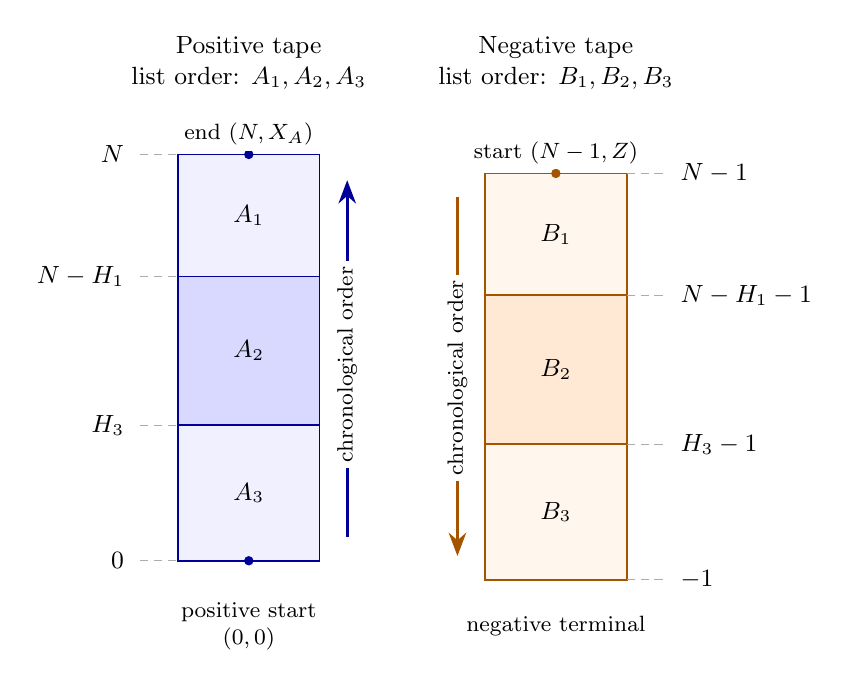
\begin{tikzpicture}[x=1cm,y=.86cm,>=Stealth,
 every node/.style={font=\small},
 posword/.style={draw=blue!60!black,fill=blue!6,line width=.6pt},
 negword/.style={draw=orange!65!black,fill=orange!7,line width=.6pt},
 guide/.style={densely dashed,gray!65,line width=.4pt}]
 \node[align=center] at (3.1,8.05)
   {Positive tape\\list order: $A_1,A_2,A_3$};
 \node[align=center] at (7.0,8.05)
   {Negative tape\\list order: $B_1,B_2,B_3$};
 \draw[posword] (2.2,.7) rectangle (4,2.7);
 \draw[posword,fill=blue!15] (2.2,2.7) rectangle (4,4.9);
 \draw[posword] (2.2,4.9) rectangle (4,6.7);
 \draw[negword] (6.1,.42) rectangle (7.9,2.42);
 \draw[negword,fill=orange!17] (6.1,2.42) rectangle (7.9,4.62);
 \draw[negword] (6.1,4.62) rectangle (7.9,6.42);
 \node at (3.1,1.7) {$A_3$};
 \node at (3.1,3.8) {$A_2$};
 \node at (3.1,5.8) {$A_1$};
 \node at (7,1.42) {$B_3$};
 \node at (7,3.52) {$B_2$};
 \node at (7,5.52) {$B_1$};
 \draw[->,very thick,blue!60!black] (4.35,1.05)--(4.35,6.32);
 \draw[->,very thick,orange!65!black] (5.75,6.07)--(5.75,.77);
 \node[rotate=90,font=\footnotesize,fill=white,inner sep=2pt]
   at (4.35,3.6) {chronological order};
 \node[rotate=90,font=\footnotesize,fill=white,inner sep=2pt]
   at (5.75,3.4) {chronological order};
 \foreach \yy/\ll in {.7/0,2.7/H_3,4.9/{N-H_1},6.7/N} {
   \draw[guide] (1.72,\yy)--(2.2,\yy);
   \node[anchor=east] at (1.64,\yy) {$\ll$};
 }
 \foreach \yy/\ll in {.42/{-1},2.42/{H_3-1},4.62/{N-H_1-1},6.42/{N-1}} {
   \draw[guide] (7.9,\yy)--(8.38,\yy);
   \node[anchor=west] at (8.46,\yy) {$\ll$};
 }
 \fill[blue!60!black] (3.1,.7) circle (1.7pt);
 \fill[blue!60!black] (3.1,6.7) circle (1.7pt);
 \fill[orange!65!black] (7,6.42) circle (1.7pt);
 \node[anchor=north,align=center,font=\footnotesize] at (3.1,.22)
   {positive start\\$(0,0)$};
 \node[anchor=north,align=center,font=\footnotesize] at (7,.02)
   {negative terminal};
 \node[anchor=south,font=\footnotesize,fill=white,inner sep=2pt]
   at (7,6.47) {start $(N-1,Z)$};
 \node[anchor=south,font=\footnotesize,fill=white,inner sep=2pt]
   at (3.1,6.75) {end $(N,X_A)$};
\end{tikzpicture}
\caption{The three chunks in the opposed arrangement, after translation
to put the positive starting site at $(0,0)$, with $N=H_1+H_2+H_3$.
Both tape lists are indexed from top to bottom. The positive path follows
chunks $3,2,1$, reversing each slab list while retaining the forward steps
of every word; the negative path follows chunks $1,2,3$ in their original
order. The one-level offset makes the departure heights in corresponding
chunks agree. Under the actual law $P^{(n)}$, the lateral gap at the top
is $Z-X_A=d_0$. The shaded middle chunks define $E_{\rm mid}$. Rectangles
show height ranges, not path traces; widths, heights, and lateral
placements are schematic.}
\label{fig:opposed-chunks}
\end{figure}


Define a second law \(Q^{(n)}\) on these same variables.  Keep the
\(P^{(n)}\)-marginal of \((H,Z)\); conditional on \((H,Z)\), sample the
six lists independently, with
\[
 A_i\sim\mathcal B_{H_i}^+,
 \qquad B_i\sim\mathcal B_{H_i}^-,
 \qquad i=1,2,3.
\]
These exact-cut bridge laws are defined by \eqref{eq:bridge-law}.
Since \(H_i\ge Mn\), their normalizing constants have the positive lower
bounds supplied by \eqref{eq:bridge-renewal}.
Thus the reference law keeps the three widths and the negative starting
position, and independently resamples the six relative lists.  The same
placement rule defines \(E_{\rm mid}\) under both laws.

\begin{proposition}[Entropy comparison]\label{prop:entropy-comparison}
For every integer \(n\ge1\), the actual chunk law and the reference law
above satisfy
\begin{equation}
 D(P^{(n)}\Vert Q^{(n)})\le C+h_{14n}'-h_n'.
 \label{eq:entropy-comparison}
\end{equation}
\end{proposition}

\begin{proof}
All entropies and expectations in this proof refer to the original
tape-and-count experiment.
First omit \(Z\), and let \(D_0\) denote the relative entropy between
the resulting marginals of \(P^{(n)}\) and \(Q^{(n)}\).  A pair of lists
of common width \(h\) determines the number of its common renewals,
counting the terminal width \(h\) and excluding zero, and hence determines
its parsing into common blocks.  If that number is in the count window
for chunk \(i\), the actual unconditioned probability of the list pair is
\[
 \frac1n
 \prod_{\gamma\in A_i}W(\gamma)
 \prod_{\gamma\in B_i}W(\gamma).
\]
If the number is outside the window, the probability is zero.  This follows
from the common-block construction and the slab weights: the specified
pair of lists determines exactly one allowed count.  In contrast, the
product of the two bridge laws at width \(h\) has the same product of
weights divided by \(\bar u_h^+\bar u_h^-\).  Thus, conditional on
\(H_i=h\), the density relative to the independent bridges is, on the
actual support, exactly
\begin{equation}
 \frac{\bar u_h^+\bar u_h^-}
      {nP^{(n)}(H_i=h)}.
 \label{eq:chunk-pair-density}
\end{equation}
Independence of the three actual chunks now gives
\begin{align}
 I(\mathcal A;\mathcal B\mid H)
 &\le D_0\notag\\
 &=\sum_{i=1}^3
   \left(\Ent(H_i)-\log n
          +\mathbb E\log(\bar u_{H_i}^+\bar u_{H_i}^-)\right)
 \le\sum_{i=1}^3(\Ent(H_i)-\log n)
 \le C.
 \label{eq:chunk-entropy-cost}
\end{align}
The information inequality follows from
\eqref{eq:conditional-product-entropy}.  For the last bound, use
\(\mathbb E H_i=\mathbf E K_1\,\mathbb E I_i=O(n)\) and compare the
law of \(H_i\) with weights proportional to \(e^{-h/n}\) on the
nonnegative integers.  The normalizer is \(O(n)\), so
\(\Ent(H_i)\le\log n+C\).

Reintroducing \(Z\) costs its conditional information with the lists:
\begin{equation}
 \begin{split}
 D(P^{(n)}\Vert Q^{(n)})
 &=D_0+I(Z;\mathcal A,\mathcal B\mid H)\\
 &=D_0+\Ent(Z\mid H)-\Ent(d_0).
 \end{split}
 \label{eq:buffer-information}
\end{equation}
Here the lists determine \(X_A\), and the buffer is independent of the
lists and widths; conditional on those data, \(Z\) is a translate of
\(d_0\).  Likewise, given \((\mathcal A,H)\), the variable \(Z\) is
conditionally independent of \(\mathcal B\).  Conditional data processing
and \eqref{eq:chunk-entropy-cost} imply
\[
 I(Z;\mathcal B\mid H)
 \le I(\mathcal A;\mathcal B\mid H)\le D_0.
\]
Every variable whose entropy is evaluated in the next calculation has
finite entropy; the conditioning lists need not:
\begin{align}
 \Ent(T,Z+X_B)
 &\ge\Ent(T,Z+X_B\mid\mathcal B,H)
   =\Ent(T,Z\mid\mathcal B,H)\notag\\
 &\ge\Ent(Z\mid H)-D_0
       +\Ent(T\mid Z,\mathcal A,\mathcal B,H)\notag\\
 &=\Ent(Z\mid H)-D_0+\Ent(I_0\mid d_0).
 \label{eq:buffer-entropy-lower}
\end{align}
For the final identity, each pair of chunk lists determines its common
block count, hence \(I_1,I_2,I_3\).  The lists and \(Z\) also determine
\(d_0=Z-X_A\).  Independence from the buffer then identifies the
remaining conditional entropy of \(T\) with \(\Ent(I_0\mid d_0)\).

Subtract \(\Ent(I_0,d_0)=\Ent(d_0)+\Ent(I_0\mid d_0)\) from
\eqref{eq:buffer-entropy-lower} and use
\eqref{eq:buffer-information}.  The result is
\begin{equation}
 D(P^{(n)}\Vert Q^{(n)})
 \le 2D_0+\Ent(T,Z+X_B)-\Ent(I_0,d_0).
 \label{eq:two-entropy-costs}
\end{equation}
Now \(Z+X_B\) is the sum of the lateral increments through the first
\(T\) common blocks.  Both \(T\) and \(I_0\) are independent of the
underlying block sequence.  It follows that
\begin{align*}
 \Ent(T,Z+X_B)-\Ent(I_0,d_0)
 &=\Ent(T)+\mathbb E h_T'-\log n-\mathbb E h_{I_0}'\\
 &\le C+h_{14n}'-h_n'.
\end{align*}
Indeed, \(T<14n\), \(I_0\ge n\), and \(T\) has at most \(4n\)
possible values.  Monotonicity of \(h_j'\) proves the displayed bound.
Finally, the term \(2D_0\) is bounded uniformly in \(n\) by
\eqref{eq:chunk-entropy-cost}, proving
\eqref{eq:entropy-comparison}.
\end{proof}

\subsection{Contacts under the reference law}

The entropy comparison will bound the contact count once we show that
\(E_{\rm mid}\) contains the relevant actual contacts and is unlikely
under the reference law.
For every realization of the counts, a contact in a positive common block
with index in \((4n,8n]\) implies \(E_{\rm mid}\).  In fact, chunk \(2\)
starts after at most \(4n-2\) common blocks and ends at or beyond block
\(9n\).  The negative departure realizing a contact is in the same or a
neighboring block, by the common-block geometry in
Section~\ref{sec:bridges}; all those blocks remain inside chunk \(2\).
Consequently
\begin{equation}
 \mathbf P\{\text{a contact in a positive block indexed in }(4n,8n]\}
 \le P^{(n)}(E_{\rm mid}).
 \label{eq:middle-contact-inclusion}
\end{equation}

\begin{proposition}[Reference contact bound]\label{prop:reference-contact}
For every integer \(n\ge1\),
\begin{equation}
 Q^{(n)}(E_{\rm mid})\le\delta_n,
 \qquad
 \delta_n=\min\{1,Cn(F_+(n)+F_-(n))\}.
 \label{eq:reference-contact}
\end{equation}
\end{proposition}

\begin{proof}
Fix \((H,Z)\) in the support of its retained marginal.  Conditional on
these data, all six reference lists are independent.  Reversing the
positive list order preserves its bridge law by
\eqref{eq:bridge-law}.  Retain the positive path formed by chunks \(3\)
and \(2\), and call it \(\alpha\).  It runs from the origin through its
first hit of height \(N-H_1\).  For the negative path formed by chunks
\(1\) and \(2\), retain only the prefix through its first arrival within
distance \(R\) of \(\Dep(\alpha)\); call the retained prefix \(\beta\)
and its terminal site \(y'\).  On \(E_{\rm mid}\) such an arrival exists
no later than a negative departure in chunk \(2\), and hence before the
two negative chunks terminate.
This first proximity need not itself join the two middle chunks; the
outer chunk widths will nevertheless put both visits at progress at
least \(n\).

The geometry puts this encounter away from both starting sides.  The two
negative chunks stay at or below \(N-1\) and end at their first hit of
\(H_3-1\).  Therefore
\[
 H_3\le y_1'\le N-1.
\]
Choose a departure \(y\) of \(\alpha\) within distance \(R\) of \(y'\).
Since \(\alpha\) ends on its first hit of \(N-H_1\),
\begin{equation}
 H_3-R\le y_1\le N-H_1-1,
 \qquad N-1-y_1'\ge H_1-R.
 \label{eq:reference-contact-heights}
\end{equation}
The inequalities \(H_1,H_3\ge Mn\) and \(M>R+1\) show that both visits
occur at or after the respective path has reached signed progress \(n\)
from its start.  Up to these visits neither path has hit either absolute
height \(-1\) or \(N\).

We next express the probability of these prefixes using two raw walks in
one environment.  The unused positive chunk \(1\) and negative chunk
\(3\) integrate to one.  The four remaining bridge normalizations,
\[
 \bar u_{H_3}^+\bar u_{H_2}^+
 \bar u_{H_1}^-\bar u_{H_2}^-,
\]
have a fixed positive lower bound by \eqref{eq:bridge-renewal}.  Within
each sign, concatenating the two bridges gives the product of their raw
weights, by the separation of active departures established in
Section~\ref{sec:bridges}.

For fixed \(\alpha\) and a retained negative prefix \(\beta\), sum over
all allowed negative completions to the terminal height \(H_3-1\).
Their total raw weight is at most \(W(\beta)\): full words to that height
end on its first hit, so the corresponding continuation events are
disjoint.  Nor is there multiplicity from the lists.  The intermediate
chunk boundary is a first hit of its prescribed height, and the bridge
parsing into slabs is unique.  The same uniqueness holds for the positive
concatenation.  Thus, after dropping any further completion restrictions,
the conditional contact probability is at most a fixed constant times a
sum of products
\begin{equation}
 W(\alpha)W(\beta)
 =\mathbb E_Q\bigl[p_\omega(\alpha)p_\omega(\beta)\bigr].
 \label{eq:reference-prefix-transfer}
\end{equation}
The equality holds for each retained pair: every departure of \(\beta\)
precedes its first proximity arrival and is therefore at distance strictly
greater than \(R\) from every departure of \(\alpha\).  The terminal
arrival \(y'\) uses no departure row.  Lemma~\ref{lem:separated-weights}
then applies, with repeated departures within either path retained in
their respective weights.

The right side of \eqref{eq:reference-prefix-transfer} is the probability
of the specified prefixes for two raw marked walks, started at \(0\) and
\((N-1,Z)\), independently conditional on a shared environment of law
\(Q\).  Summing these probabilities introduces no overcounting.  A full
positive trajectory has at most one prefix through its first hit of the
fixed height \(N-H_1\); that prefix determines \(\Dep(\alpha)\), and a
full negative trajectory has at most one prefix through its first arrival
within distance \(R\) of that set.

Only in this shared-environment experiment do we classify an encounter by
quenched exit probabilities.  For \(0\le x_1\le N-1\), define
\[
 q_x^\omega=P_{x,\omega}(T_{-1}<T_N),
\]
where \(T_a\) here is the first hit of absolute first-coordinate height
\(a\).  Slab exit is almost surely finite, so
\(1-q_x^\omega=P_{x,\omega}(T_N<T_{-1})\).  At the sites in
\eqref{eq:reference-contact-heights}, if \(q_y^\omega\ge1/2\), the
positive walk has visited, after reaching progress \(n\), a site with
probability at least \(1/2\) of exiting through its starting side's
barrier \(-1\).  If \(q_y^\omega<1/2\), join \(y'\) to \(y\) by a
coordinate path of at most \(dR\) steps inside the slab.  Uniform
ellipticity gives
\[
 1-q_{y'}^\omega
 \ge\kappa^{dR}(1-q_y^\omega)
 \ge\kappa^{dR}/2.
\]
In that case the negative walk has visited, after reaching its signed
progress \(n\), a site with probability at least \(\kappa^{dR}/2\) of
exiting through its own starting side's barrier \(N\).

For either sign \(\sigma\), consider the raw marginal event that, after
its first hit of signed progress \(n\) and before slab exit, the walk
visits a site whose quenched probability of exit through the starting
side's barrier is at least \(c=\kappa^{dR}/2\).  With the environment
fixed, stop at the first such visit.  The probability of the indicated
exit after this visit is at least \(c\).  Integrating the resulting
inequality over environments bounds the visit probability by
\begin{equation}
 c^{-1}(u_n^\sigma-u_N^\sigma).
 \label{eq:reference-visit-bound}
\end{equation}
Indeed, from each of the two starting sites, the barriers have signed
relative heights \(-1,N\).  The difference
\(u_n^\sigma-u_N^\sigma\) is exactly the raw probability of hitting
signed height \(n\) and then exiting at \(-1\) before \(N\): a path
reaching \(N\) must first reach \(n\), and exit from the finite slab is
almost surely finite.  Stationarity identifies the negative walk's
translated raw probabilities with \(u_n^-,u_N^-\).

Every retained pair belongs to at least one of these two raw visit events.
Combining \eqref{eq:reference-prefix-transfer}--\eqref{eq:reference-visit-bound}
therefore gives
\[
 Q^{(n)}(E_{\rm mid}\mid H,Z)
 \le C\sum_{\sigma\in\{+,-\}}(u_n^\sigma-u_N^\sigma)
 \le CN(F_+(n)+F_-(n)),
\]
where the last inequality is Lemma~\ref{lem:width-tail}.  This estimate
uses the raw marginal visit probabilities after the prefix transfer; it
does not condition an exit probability on the contact event.  Finally,
the retained marginal has
\[
 \mathbb E N=\mathbf E K_1\,\mathbb E(I_1+I_2+I_3)=O(n).
\]
Averaging over \((H,Z)\) and also using the trivial probability bound
one proves \eqref{eq:reference-contact}.
\end{proof}

\subsection{Summing over scales}

\begin{proposition}[Contact upper bound]\label{prop:contact-upper}
For the two independent opposed tapes under coordinate coexistence, the
contact count defined in \eqref{eq:contact-count} satisfies
\begin{equation}
 m(J)=O\!\left(\frac{J}{\log J}\right)
 \qquad(J\to\infty).
 \label{eq:contact-upper}
\end{equation}
\end{proposition}

\begin{proof}
Apply data processing in Proposition~\ref{prop:entropy-comparison} to
the indicator of \(E_{\rm mid}\).  If \(p=P^{(n)}(E_{\rm mid})\) and
\(q_n=Q^{(n)}(E_{\rm mid})\), binary relative entropy satisfies
\[
 D(\operatorname{Bern}(p)\Vert\operatorname{Bern}(q_n))
 \ge p\log(1/q_n)-\log2.
\]
Together with Proposition~\ref{prop:reference-contact}, this yields, when
\(\delta_n>0\),
\begin{equation}
 P^{(n)}(E_{\rm mid})\log(1/\delta_n)
 \le C+h_{14n}'-h_n'.
 \label{eq:contact-entropy-price}
\end{equation}
If \(\delta_n=0\), then \(q_n=0\), and the finite relative entropy in
\eqref{eq:entropy-comparison} forces
\(P^{(n)}(E_{\rm mid})=0\).  The same observation handles \(q_n=0\)
when \(\delta_n>0\).

For \(l\ge2\), take \(n=2^{l-2}\).  The width-tail summability in
Lemma~\ref{lem:width-tail} implies
\[
 \sum_{l\ge2}\delta_{2^{l-2}}<\infty.
\]
Among \(2\le l\le J\), at most \(O(\sqrt J)\) indices can have
\(\delta_{2^{l-2}}>J^{-1/2}\).  At every other index with positive
\(\delta_{2^{l-2}}\), the logarithm in
\eqref{eq:contact-entropy-price} is at least \(\tfrac12\log J\).
The corresponding entropy differences have a telescoping bound:
\begin{align*}
 \sum_{l=2}^J
   \bigl(h_{14\cdot2^{l-2}}'-h_{2^{l-2}}'\bigr)
 &\le\sum_{l=2}^J
   \bigl(h_{2^{l+2}}'-h_{2^{l-2}}'\bigr)\\
 &\le4h_{2^{J+2}}'=O(J),
\end{align*}
by monotonicity and \eqref{eq:lateral-entropy-bound}.  Since
\((4n,8n]=(2^l,2^{l+1}]\), use
\eqref{eq:middle-contact-inclusion}, sum
\eqref{eq:contact-entropy-price} over the remaining indices, and bound
each exceptional probability by one.  Adding the initial scale gives
\[
 m(J)\le 1+O(\sqrt J)+O(J/\log J)=O(J/\log J),
\]
as claimed.
\end{proof}

\section{First contacts near an aligned endpoint}\label{sec:posteriors}

Proposition~\ref{prop:contact-upper} bounds the number of scales at which
the opposed tapes meet.  To obtain a competing lower bound, we consider a
positive bridge and a relative negative path sampled independently of
it.  We place the negative path one level below the bridge's endpoint.
The bridge's final scripted departure is exactly the
negative starting site, so there is always a contact one level below
the endpoint.  We shall show that,
after a prescribed script at a lower height, their first contact is
unlikely to be delayed until much higher up the bridge.

The lateral starting point of the negative path is determined by the
positive endpoint.  We keep this dependence in the conditional
probabilities of the possible endpoints, and estimate their running
maxima together.  The martingale and endpoint-posterior arguments below
adapt \cite[Lemma~6.1 and Proposition~6.2]{OpenAI2026}.  The following
lemma gives the needed bound.

\begin{lemma}[Maxima of a finite martingale family]\label{lem:posterior-max}
Let \(m\ge1\), and let \((w_i(e))_{i\ge0}\), \(1\le e\le m\), be
nonnegative martingales for the same filtration \((\mathcal F_i)_{i\ge0}\), with
\(\sum_{e=1}^m w_i(e)\le1\) almost surely for every \(i\).  Set
\[
 A_i(e)=\max_{0\le j\le i}w_j(e),\qquad
 A_i=\sum_{e=1}^m A_i(e),\qquad
 A_\infty=\lim_{i\to\infty}A_i,
 \qquad B=\log(m+1).
\]
Write also \(A_\infty(e)=\lim_i A_i(e)\).
There are absolute constants \(c,C>0\) such that
\begin{equation}\label{eq:posterior-exponential}
 \EE\exp(cA_\infty/B)\le C.
\end{equation}
Moreover, on any joint probability space with this martingale marginal,
every event \(V\) of probability \(p\) satisfies
\begin{equation}\label{eq:event-weighted-max}
 \EE[A_\infty\one_V]
 \le CBp\log(\mathrm e/p),
\end{equation}
where the right-hand side is defined to be zero at \(p=0\).
The event \(V\) need not belong to the martingale filtration.
\end{lemma}

The logarithmic first-moment bound underlying this lemma follows by
coordinatewise integration of the scalar maximal inequality; the same
posterior calculation appears in
\cite[Section~1.1]{KesselheimMolinaroPattonSingla2026}.
The passage from bounded conditional future increases to exponential
integrability is related to the energy inequalities for increasing
processes in \cite[Theorem~4 and its corollary]{Kikuchi1992}.
We give a direct threshold proof.

\begin{proof}
Fix a time \(i\).  Conditional on the filtration at that time, the
nonnegative-martingale maximal inequality
\cite[Chapter~V, first section, \S2, Theorem~1]{Ville1939}
bounds the probability that
coordinate \(e\) subsequently exceeds \(u>0\) by \(w_i(e)/u\).
For completeness, on a finite horizon this follows by stopping at the
first crossing, using the martingale identity and nonnegativity on the
complement of the crossing event; increasing the horizon gives the
infinite-horizon bound.  Since each coordinate is at most one,
integration over \(u\in[A_i(e),1]\) gives
\[
 \EE[A_\infty(e)-A_i(e)\mid\mathcal F_i]
 \le w_i(e)\log\frac1{A_i(e)}
 \le w_i(e)\log\frac1{w_i(e)}.
\]
If \(w_i(e)=0\), its future values vanish almost surely conditionally,
and the expected increase is zero.  Add the missing mass
\(1-\sum_e w_i(e)\) to form a probability vector.  Its entropy is at
most \(\log(m+1)\), so
\begin{equation}\label{eq:maximum-remaining-increase}
 \EE[A_\infty-A_i\mid\mathcal F_i]\le B.
\end{equation}

We also have \(A_0\le1\) and
\(A_i-A_{i-1}\le\sum_e w_i(e)\le1\).
Consider the thresholds \(b_j=1+j(2B+1)\), \(j\ge1\).
The probability of strictly crossing the first threshold is at most
\(1/2\), by \eqref{eq:maximum-remaining-increase} and Markov's
inequality.  At the first crossing of any threshold, the overshoot is
at most one.  Crossing the next threshold therefore requires a further
increase greater than \(2B\), whose conditional probability is at most
\(1/2\).  This argument at a crossing time follows by splitting over
its possible finite values.  It gives a geometric tail for
\(A_\infty\) at the thresholds \(b_j\), and hence
\eqref{eq:posterior-exponential}.

For \(p>0\), conditional Jensen gives
\[
 \exp\!\left(\frac cB\EE[A_\infty\mid V]\right)
 \le \EE[\exp(cA_\infty/B)\mid V]\le C/p.
\]
Taking logarithms and multiplying by \(p\) proves
\eqref{eq:event-weighted-max}, after changing the absolute constant.
\end{proof}

We now formulate the first-contact estimate.  For a path in absolute
coordinates, write \(T_j\) for its first hit of the hyperplane
\(\{x:x_1=j\}\), specifying the path when needed.  Recall that
\(\mathcal B_N^+\) is the positive exact-cut bridge law: its
concatenated path has the raw marked law through \(T_N\), conditioned
on \(\mathcal D_N^+\).  The event \(\mathcal D_k^+\) prescribes the
\(M\)-step script immediately after the first hit of \(k-M\), reached
before height \(-1\).

\begin{proposition}[First contact above a scripted prefix]
\label{prop:first-contact}
Assume \(p_+p_->0\), and let \(M\le k<r<N\) be integers with
\(r-k\ge R\).  Start a positive bridge \(Y\) with law
\(\mathcal B_N^+\) at the origin, and put
\(E_{\mathrm{lat}}=\pi Y_{T_N}\).
Independently of \(Y\), sample a relative marked path with law
\(\widehat P_-\), and translate it to start at
\((N-1,E_{\mathrm{lat}})\); denote the resulting path by \(\beta\).
Define
\[
 \tau=\inf\{i:T_k(Y)\le i<T_N(Y),\quad
       \|Y_i-\beta_j\|_\infty\le R\text{ for some }j\ge0\},
\]
with \(\inf\varnothing=\infty\).  Let
\begin{equation}\label{eq:first-contact-event}
 \mathcal C_{k,r,N}=
 \left\{
 \begin{gathered}
  \mathcal D_k^+(Y),\quad \tau<T_N(Y),\quad (Y_\tau)_1\ge r,\\
  \min_{T_k(Y)\le i\le\tau}(Y_i)_1\ge k,
  \quad |E_{\mathrm{lat}}|\le N^2
 \end{gathered}
 \right\}.
\end{equation}
Here \(\mathcal D_k^+(Y)\) is a condition on the prefix through the
first hit of \(k\).  There is a constant \(C\), independent of
\(k,r,N\), such that, with
\(\Delta=u_{r-k}^+-u_{N-k}^+\),
\begin{equation}\label{eq:first-contact-bound}
 P(\mathcal C_{k,r,N})
 \le C\log(2N)\,\Delta\log^2(\mathrm e/\Delta).
\end{equation}
The right-hand side is defined to be zero when \(\Delta=0\).
\end{proposition}

The small parameter in this estimate is controlled by the width tail:
Lemma~\ref{lem:width-tail} gives
\[
 \Delta\le C(N-r)F_+(r-k).
\]
Thus the remaining height \(N-r\) is compared with the width tail at
the progress \(r-k\) already made above the scripted prefix.

\begin{proof}
We first express the event using finite positive prefixes and the full
negative path.  This permits a comparison in a shared environment
without treating \(\tau\) as a stopping time.  The endpoint
conditional probabilities remain attached to the positive prefixes;
Lemma~\ref{lem:posterior-max} will control their contribution.

\emph{Prefix probabilities.}
Let
\[
 \mathcal E_N=\{e\in\ZZ^{d-1}:|e|\le N^2\}.
\]
Enumerate the marked prefixes \(a_0\) that realize
\(\mathcal D_k^+\), ending at their first hit \(z\) of height \(k\).
For each such \(a_0\), enumerate all finite marked words \(a\) from
\(z\) whose vertices have heights in \([k,N-1]\) and whose terminal
site \(y=y(a)\) has height at least \(r\).
For a marked prefix \(c\) and \(e\in\mathcal E_N\), define
\begin{equation}\label{eq:endpoint-prefix-posterior}
 w(c;e)=P_0\bigl(\mathcal D_N^+,\ \pi X_{T_N}=e
                  \mid X\text{ with marks begins with }c\bigr).
\end{equation}
This is a deterministic function of \(c\) and \(e\).
All active departures in \(a_0\) lie strictly below height \(k-M\),
whereas all departures in \(a\) have height at least \(k\).
Lemma~\ref{lem:separated-weights} therefore gives
\[
 W(a_0a)=W(a_0)W(a).
\]
Consequently the raw probability of the prefix \(a_0a\) and the
endpoint event in \eqref{eq:endpoint-prefix-posterior} is
\(W(a_0)W(a)w(a_0a;e)\).

For a raw negative path starting at \((N-1,e)\), let \(D^-\) denote
the event that all its heights are at most \(N-1\).
Let \(\mathcal V(a)\) be the event that this path satisfies \(D^-\),
avoids the closed \(R\)-neighborhood of \(\Dep(a)\) for all time,
and visits the closed \(R\)-neighborhood of \(y(a)\).
Thus \(\mathcal V(a)\) asserts that the first contact along the word
\(a\) occurs at its terminal site.  If that site was an earlier
departure of \(a\), the event is empty.
The raw bridge interpretation and the conditioning by \(D^-\) give
the exact identity
\begin{equation}\label{eq:first-contact-prefix-sum}
 \begin{split}
 P(\mathcal C_{k,r,N})
 =\frac1{\bar u_N^+p_-}
 \sum_{a_0}W(a_0)
 \sum_{e\in\mathcal E_N}\sum_a
 W(a)w(a_0a;e)P_{(N-1,e)}(\mathcal V(a)).
 \end{split}
\end{equation}
Indeed, a pair of paths in \(\mathcal C_{k,r,N}\) determines a unique
\(a_0\) and a unique prefix \(a\) ending at its first contact after
\(T_k\).  Conversely every term represents exactly these conditions.
All word families are countable, and every summand is nonnegative.

\emph{A shared environment for the unconditioned prefixes.}
Fix \(a_0\) for the moment.  For a word \(a\), put
\[
 B(a)=\{x\in\ZZ^d:\dist_\infty(x,\Dep(a))\le R\}.
\]
The quenched probability of \(\mathcal V(a)\) can be computed from
the negative walk killed on arrival in \(B(a)\).  It requires eternal
survival, the upper-height restriction, and a visit near \(y(a)\).
It therefore uses only rows in \(B(a)^c\), including when these
requirements concern the entire infinite path.  Those rows are more
than distance \(R\) from every active departure of \(a\).
Finite-range independence gives
\begin{equation}\label{eq:first-contact-transfer}
 W(a)P_{(N-1,e)}(\mathcal V(a))
 =E_Q\left[p_\omega(a)
           P_{(N-1,e),\omega}(\mathcal V(a))\right].
\end{equation}

The right-hand side has the following interpretation.  Sample a fresh
environment with law \(Q\).  In it, run a raw comparison path
\(\widetilde X\) from \(z\) and a raw negative path
\(\widetilde\beta^{\,e}\) from \((N-1,e)\), independently
conditional on the environment.  Denote its law and expectation by
\(P_e^{\mathrm c},E_e^{\mathrm c}\), and write
\(P^{\mathrm c},E^{\mathrm c}\) for the common
\((\omega,\widetilde X)\) marginal, which does not depend on \(e\).
For fixed \(a_0,e\), the inner sum in
\eqref{eq:first-contact-prefix-sum} becomes
\begin{equation}\label{eq:transferred-prefix-sum}
 E_e^{\mathrm c}\left[
  \sum_a w(a_0a;e)
  \one_{\{\widetilde X\text{ begins with }a\}}
  \one_{\{\widetilde\beta^{\,e}\in\mathcal V(a)\}}
 \right].
\end{equation}
For every realized pair, at most one summand is nonzero: its terminal
site must be the first site of \(\widetilde X\) within distance
\(R\) of the full range of \(\widetilde\beta^{\,e}\).
This uniqueness is a pathwise fact and uses no stopping-time property
of the first contact.

\emph{The stopped posterior law.}
The factors \(w(a_0a;e)\) in
\eqref{eq:transferred-prefix-sum} still come from the original raw
positive law conditioned on \(a_0\).  In that law, let
\(\mathcal G_i\) record the marked continuation for \(i\) steps,
and form the martingales
\[
 w_i(e)=P_0(\mathcal D_N^+,\ \pi X_{T_N}=e
                  \mid a_0,\mathcal G_i),
 \qquad e\in\mathcal E_N.
\]
They are nonnegative and have sum at most one.  Stop the continuation
on its first hit of height \(k-1\) or \(N\).  Every departure before
that stop has height at least \(k\), so it is separated from the
active departures of \(a_0\).  The stopping arrival uses no row.
By factoring each finite stopped-prefix probability, the conditional
stopped continuation therefore has exactly the same path law as
\(\widetilde X\) stopped at
\[
 \zeta=T_{k-1}(\widetilde X)\wedge T_N(\widetilde X).
\]
Both stops are almost surely finite by uniform ellipticity and exit
from a slab of bounded height.

Evaluate the same deterministic functions
\eqref{eq:endpoint-prefix-posterior} along the comparison path until
\(\zeta\), and freeze them afterwards.  More explicitly, if
\(\widetilde X_{[0,j]}\) denotes its marked prefix of length \(j\),
set
\[
 \widetilde w_i(e)
 =w\bigl(a_0\widetilde X_{[0,i\wedge\zeta]};e\bigr).
\]
Equality of the stopped path laws shows that this vector has the
stopped martingale law just described.  Its values remain the original
conditional probabilities given \(a_0\); they are not conditional
probabilities given the fresh environment.  In particular, the value
at a hit of \(k-1\) retains its original meaning, and no identification
of continuation laws beyond that hit is needed.

Define
\[
 M_*(e)=\max_{0\le i\le\zeta}\widetilde w_i(e),
 \qquad S_*=\sum_{e\in\mathcal E_N}M_*(e).
\]
All endpoint coordinates are functions of the same stopped comparison
path.  We can therefore estimate their sum \(S_*\) on an event while
retaining only a logarithmic dependence on the number of endpoints.
Applying Lemma~\ref{lem:posterior-max} and using
\(\log(|\mathcal E_N|+1)\le C\log(2N)\) gives, for any event \(V\)
depending on the comparison path and its environment,
\begin{equation}\label{eq:stopped-posterior-event}
 E^{\mathrm c}[S_*\one_V]
 \le C\log(2N)\,P^{\mathrm c}(V)
                  \log\frac{\mathrm e}{P^{\mathrm c}(V)}.
\end{equation}
The constant is uniform over \(a_0\).  We have thus controlled the
endpoint factors while preserving a fresh shared environment in which
to estimate contacts.

\emph{Quenched exit probabilities.}
For an interior site \(y\), meaning \(k\le y_1<N\), write
\[
 q_y^\omega=P_{y,\omega}(T_{k-1}<T_N).
\]
Ellipticity gives \(0<q_y^\omega<1\).  For
\(t=2^{-j}\), \(j\ge1\), let \(V_t\) be the event that
\(\widetilde X\), at or after its first hit of height \(r\) and
before \(\zeta\), visits a site with \(q_y^\omega\ge t\).
With the environment fixed, stop at the first such visit.  The
conditional chance of exiting at \(k-1\) is then at least \(t\).
After averaging, stationarity and almost sure slab exit give
\begin{equation}\label{eq:first-contact-large-q}
 \begin{split}
 tP^{\mathrm c}(V_t)
 &\le P_z(T_r<T_{k-1}<T_N)\\
 &=u_{r-k}^+-u_{N-k}^+=\Delta.
 \end{split}
\end{equation}

Suppose a retained prefix ends at \(y\) with
\(q_y^\omega\in[t,2t)\).  Its endpoint lies at height at least
\(r\), so \(V_t\) occurs.  The negative path visits a site \(y'\)
within distance \(R\) of \(y\).  Because \(r-k\ge R\) and the
negative path satisfies \(D^-\), this site is also interior:
\(k\le y'_1\le N-1\).  A coordinate path from \(y\) to \(y'\)
of length at most \(dR\) stays inside the slab.  Following this path
and then exiting through the lower boundary shows that
\[
 q_y^\omega\ge\kappa^{dR}q_{y'}^\omega,
 \qquad q_{y'}^\omega\le c_Rt,
 \qquad c_R=2\kappa^{-dR}.
\]

For each fixed environment, the probability that a raw path from
\((N-1,e)\) satisfies \(D^-\) and visits any interior site with
\(q_{y'}^\omega\le c_Rt\) is at most \(c_Rt\), uniformly in \(e\).
Indeed, stop on the first visit to that set.  To satisfy \(D^-\)
after this visit, the path must next leave the slab through \(k-1\),
except on the null event of never exiting it.  The strong Markov property
bounds the conditional probability of this next exit by
\(q_{y'}^\omega\le c_Rt\) at the first-visit site, regardless of
earlier visits below \(k-1\).

\emph{Summing the exit-probability bins.}
We classify the transferred sum
\eqref{eq:transferred-prefix-sum} according to
\(q_{y(a)}^\omega\in[t,2t)\).  This classification is made in the
shared environment, after \eqref{eq:first-contact-transfer} has been
applied.  A retained prefix ends before \(\zeta\), so its posterior
factor is at most \(M_*(e)\).  By uniqueness of the retained prefix,
its contribution in this bin is pointwise bounded by \(M_*(e)\)
times the indicators of \(V_t\) and of the negative-path event in
the preceding paragraph.  Conditional on the environment, that
negative path is independent of \(\widetilde X\), and its event has
probability at most \(c_Rt\).  Summing over \(e\), whose comparison
path and environment have the same marginal, bounds this bin's total
contribution for fixed \(a_0\) by
\begin{equation}\label{eq:first-contact-bin}
 Ct\,E^{\mathrm c}[S_*\one_{V_t}].
\end{equation}

If \(\Delta=0\), \eqref{eq:first-contact-large-q} makes every term
zero.  Suppose \(\Delta>0\).  For \(t<\Delta\), use
\(E^{\mathrm c}S_*\le C\log(2N)\) and sum the geometric series in
\(t\).  The contribution is at most \(C\log(2N)\Delta\).
For \(t\ge\Delta\), combine
\eqref{eq:stopped-posterior-event} and
\eqref{eq:first-contact-large-q}.  Since
\(p\mapsto p\log(\mathrm e/p)\) is increasing on \([0,1]\), each
such bin contributes at most
\[
 C\log(2N)\,\Delta\log(\mathrm e t/\Delta).
\]
There are \(O(\log(\mathrm e/\Delta))\) bins in this second range,
so all bins together contribute at most
\(C\log(2N)\Delta\log^2(\mathrm e/\Delta)\).
Finally, the first-hit prefixes \(a_0\) are disjoint, hence
\(\sum_{a_0}W(a_0)\le1\), and
\eqref{eq:bridge-renewal} gives
\(\bar u_N^+p_-\ge\xi p_+p_->0\).
Substitution in \eqref{eq:first-contact-prefix-sum} proves
\eqref{eq:first-contact-bound}.
\end{proof}

\section{Contacts at many depths and completion of the proof}
\label{sec:contact-lower}

We continue to assume coexistence in the coordinate direction and adapt the
cut-averaging argument of \cite[Proposition~7.1]{OpenAI2026} to scripted cuts
and positive-side proximity labels.  The first-contact estimate from
Proposition~\ref{prop:first-contact} forces contacts in most groups
of consecutive dyadic depth intervals.  We will first count these intervals and
then use the finite mean width of the common blocks to convert depths into block
indices.  The resulting lower bound contradicts
Proposition~\ref{prop:contact-upper}.

\begin{proposition}[Contact lower bound]\label{prop:contact-lower}
Suppose that $P_0(A_{e_1})>0$ and $P_0(A_{-e_1})>0$, and let $m(J)$ be the
contact statistic of the opposed tapes defined in \eqref{eq:contact-count}.
There are constants $c>0$ and an integer $c_1\ge0$ such that, for all sufficiently
large integers $J$,
\begin{equation}\label{eq:contact-lower}
 m(J+c_1)\ge \frac{cJ}{1+\log\log J}.
\end{equation}
\end{proposition}

\begin{proof}
All constants in this proof may depend on the fixed environment law and the
marked construction, but not on $J$ or the depth parameters.  Recall that the
depth of a contact is the depth of its positive departure.  For an integer
$l\ge0$, call $l$ a \emph{contact depth label} if there is a contact at an integer
depth in $[2^l,2^{l+1})$.

\paragraph{Conditioning on a distant cut.}
Fix a large integer $J$, and set
\begin{equation}\label{eq:lower-scales}
 N=2^{2J},\qquad
 G=\left\lceil 4\log_2\log(2+J)\right\rceil+3.
\end{equation}
Let $\mathcal C_N$ be the event that $N$ is a width renewal of the positive
tape, and write
\[
 \mathbf Q_N=\mathbf P(\,\cdot\mid\mathcal C_N).
\]
By \eqref{eq:bridge-renewal},
\begin{equation}\label{eq:lower-conditioning}
 \mathbf P(\mathcal C_N)=\bar u_N^+\ge\xi p_+>0.
\end{equation}
Under $\mathbf Q_N$, follow the placed positive words from bottom to top by
reversing the order of the slab list through this renewal, without reversing
any word, and translate its bottom endpoint to the origin.  The product formula
\eqref{eq:bridge-law} is invariant under this list
reversal.  Thus the resulting chronological path $Y$ has bridge law
$\mathcal B_N^+$.  If $E_{\rm lat}=\pi Y_{T_N}$, the same translation puts the
negative tape at $(N-1,E_{\rm lat})$.  Write $\beta$ for this translated path.
Its displacement path from its starting site has law $\widehat P_-$ and is
independent of the positive list.  This is
exactly the pair of paths in Proposition~\ref{prop:first-contact}.  In these
coordinates the depth of a positive departure at $y$ is $N-y_1$.

On $\mathcal C_N$, at most $N$ positive slabs are used before width $N$, since
each width is at least $M\ge1$.  The norm of $E_{\rm lat}$ is bounded by the sum
of their radii, and hence by the sum of the first $N$ radii of the unconditioned
positive tape.  Proposition~\ref{prop:radius-moment},
\eqref{eq:lower-conditioning}, and Markov's inequality give
\begin{equation}\label{eq:lower-endpoint-tail}
 \mathbf Q_N\{\abs{E_{\rm lat}}>N^2\}\le \frac{C}{N}.
\end{equation}

\paragraph{An interval without contacts forces a late first contact.}
For $G<l\le J$, let $U_l'$ be the event that none of
$l-G,l-G+1,\ldots,l$ is a contact depth label.  We will show that
\begin{equation}\label{eq:uncovered-labels}
 \sum_{l=G+1}^J\mathbf Q_N(U_l')=o(J).
\end{equation}
Consider the possible positive cut depths
\[
 \mathcal I_l=[2^l,\tfrac32\,2^l]\cap\ZZ.
\]
For $s\in\mathcal I_l$, put
\begin{equation}\label{eq:lower-contact-parameters}
 k=N-s,\qquad r=N-2^{l-G}.
\end{equation}
For all sufficiently large $J$, these integers satisfy
$M\le k<r<N$ and $r-k\ge R$, uniformly over the indicated $l,s$.

Suppose first that $s$ is an actual cut depth of the positive tape.  In the
reversed list, its boundary is at height $k$.  Every preceding word remains
strictly below its terminal height until its final arrival, and that arrival
ends a record script.  Consequently the bridge first reaches $k$ along a
prefix realizing $\mathcal D_k^+$: it first hits $k-M$ and then follows the
prescribed $M$-step script.  All the subsequent words remain at or above $k$.
These assertions hold for the concatenated bridge, because a word's initial
boundary is a strict record of the preceding words and no script can straddle
a boundary at which another script ends.

The final positive departure before $T_N$ is $(N-1,E_{\rm lat})$, the initial
site of $\beta$.  There is therefore a first contact along $Y$ between $T_k$
and $T_N$.  Its depth is at most $s$.  On $U_l'$, there are no contacts at any
depth in $[2^{l-G},2^{l+1})$; since $s<2^{l+1}$, this first contact must have
depth less than $2^{l-G}$.  Its height is in particular at least $r$.  If also
$\abs{E_{\rm lat}}\le N^2$, all the requirements of
\eqref{eq:first-contact-event} are now satisfied.

For each \emph{deterministic} $s\in\mathcal I_l$, let $\mathcal A_{l,s}$ denote
the event \eqref{eq:first-contact-event} with the parameters
\eqref{eq:lower-contact-parameters}.  This event includes the prefix condition
$\mathcal D_k^+$, but we do not additionally require $s$ to be a cut of the
tape.  Thus Proposition~\ref{prop:first-contact} applies directly under
$\mathbf Q_N$, and gives
\begin{equation}\label{eq:lower-deterministic-cut}
 \mathbf Q_N(\mathcal A_{l,s})
 \le C\log(2N)\,\phi(\Delta_{l,s}),\qquad
 \Delta_{l,s}=u^+_{s-2^{l-G}}-u_s^+,
\end{equation}
where
\[
 \phi(x)=x\log^2(\mathrm e/x)\quad(0<x\le1),\qquad \phi(0)=0.
\]
Here and below $\mathrm e=\exp(1)$.  Lemma~\ref{lem:width-tail} implies
\begin{equation}\label{eq:lower-delta-tail}
 \Delta_{l,s}\le C2^{-G}a_l,\qquad
 a_l=2^l F_+(2^{l-1}),\qquad
 A:=\sum_{l\ge1}a_l<\infty,
\end{equation}
because $s-2^{l-G}\ge2^{l-1}$.
The factor $2^{-G}$ is the ratio between the remaining contact depth
$2^{l-G}$ and the cut depth scale $2^l$.

\paragraph{Averaging over the cut locations.}
Let $C_+(t)$ count the positive width renewals in $(0,t]$.  The positive widths
are iid with finite mean by Propositions~\ref{prop:cut-law}
and~\ref{prop:mean-width}; their strong law gives
$C_+(t)=t/E_{\nu_+}L+o(t)$ almost surely.  It follows that the number of positive
cuts in $\mathcal I_l$ is
\[
 \frac{2^{l-1}}{E_{\nu_+}L}+o(2^l)
 \quad\text{almost surely as }l\longrightarrow\infty.
\]
Fix $0<c_0<1/(2E_{\nu_+}L)$, and let $\mathcal T_J$ be the event that every
$\mathcal I_l$ with $G<l\le J$ contains at least $c_0 2^l$ positive cuts.  On
almost every tape the displayed asymptotic supplies this bound for all
sufficiently large $l$.  Since $G\to\infty$,
\[
 \mathbf P(\mathcal T_J^c)\longrightarrow0,
 \qquad
 \mathbf Q_N(\mathcal T_J^c)
 \le\frac{\mathbf P(\mathcal T_J^c)}{\xi p_+}\longrightarrow0.
\]
In particular, no convergence rate in the strong law is needed for the
changing conditional law $\mathbf Q_N$.

Every cut counted in $\mathcal I_l$ lies before depth $N$.  On $U_l'$,
$\mathcal T_J$, and $\{\abs{E_{\rm lat}}\le N^2\}$, each of these cuts supplies
one of the events $\mathcal A_{l,s}$ by the preceding argument.  We obtain the
pointwise inequality
\begin{equation}\label{eq:cut-averaging}
 \one_{U_l'}\one_{\mathcal T_J}\one_{\{\abs{E_{\rm lat}}\le N^2\}}
 \le\frac{1}{c_0 2^l}\sum_{s\in\mathcal I_l}\one_{\mathcal A_{l,s}}.
\end{equation}
The right side involves only the deterministic-parameter probabilities already
bounded in \eqref{eq:lower-deterministic-cut}.

We next sum those bounds using only $\sum_l a_l<\infty$.  For large $J$,
$C2^{-G}a_l\le\mathrm e^{-1}$ uniformly in $l$, and $\phi$ is increasing on
$[0,\mathrm e^{-1}]$.  Hence \eqref{eq:lower-delta-tail} yields
\begin{equation}\label{eq:lower-phi}
 \phi(\Delta_{l,s})
 \le C2^{-G}a_l\bigl((G+1)^2+\log_+^2(1/a_l)\bigr),
\end{equation}
where $\log_+ x=\max\{0,\log x\}$ and the right side is interpreted as zero
when $a_l=0$.  Moreover,
\begin{equation}\label{eq:lower-slow-tail}
 \sum_{l=1}^J a_l\log_+^2(1/a_l)
 \le C(A+J^{-1})\log^2 J.
\end{equation}
Indeed, terms with $a_l\ge J^{-2}$ contribute at most $4A\log^2 J$.
For the remaining terms, the function $x\log^2(1/x)$ is increasing on
$[0,J^{-2}]$ for large $J$, so each is at most $4J^{-2}\log^2 J$.

Taking expectations in \eqref{eq:cut-averaging}, using
$|\mathcal I_l|\le2^l$, and applying
\eqref{eq:lower-endpoint-tail}, \eqref{eq:lower-deterministic-cut},
\eqref{eq:lower-phi}, and \eqref{eq:lower-slow-tail}, we obtain
\begin{align}
 \sum_{l=G+1}^J\mathbf Q_N(U_l')
 &\le J\mathbf Q_N(\mathcal T_J^c)+\frac{CJ}{N}\notag\\
 &\quad+C\log(2N)\,2^{-G}
       \bigl(A(G+1)^2+(A+J^{-1})\log^2 J\bigr)
 =o(J).\label{eq:lower-uncovered-bound}
\end{align}
For the final equality, the first term is $o(J)$, while
\eqref{eq:lower-scales} gives $\log(2N)=O(J)$,
$2^{-G}=O((\log J)^{-4})$, and $G=O(\log\log J)$.
The last term is therefore $O(J/(\log J)^2)$, and $CJ/N=o(J)$.  This proves
\eqref{eq:uncovered-labels}, even when the summable sequence $(a_l)$ decays
arbitrarily slowly.

There are $J-G$ tested labels $l$.  By \eqref{eq:uncovered-labels} and Markov's
inequality, with $\mathbf Q_N$-probability tending to one, at least $J/2$ of
these tests have $U_l'$ false.  Each such test has a contact depth label in
$\{l-G,\ldots,l\}$, and any one contact label can account for at most $G+1$
tests.  Thus, if $\mathcal E_J$ is the event that at least $J/(2(G+1))$ of
$1,\ldots,J$ are contact depth labels, then
\begin{equation}\label{eq:lower-unconditioning}
 \mathbf Q_N(\mathcal E_J)\longrightarrow1,
 \qquad
 \liminf_{J\to\infty}\mathbf P(\mathcal E_J)\ge\xi p_+>0.
\end{equation}
The second assertion follows by intersecting $\mathcal E_J$ with
$\mathcal C_N$ and using \eqref{eq:lower-conditioning}.  We have therefore
obtained the needed number of depth labels under the original tape law.

\paragraph{From depths to common-block indices.}
By Proposition~\ref{prop:common-blocks}, $\mu=\mathbf E K_1$ is finite and positive,
and $W_i'/i\to\mu$ almost surely.  For an integer depth $z\ge1$, let $i(z)$ be
its common-block index, so that
\[
 W_{i(z)-1}'<z\le W_{i(z)}'.
\]
The strong law implies, almost surely for all sufficiently large integer $z$,
\begin{equation}\label{eq:depth-index-comparison}
 \frac{z}{2\mu}\le i(z)<\frac{2z}{\mu}+1.
\end{equation}
Consequently there is a deterministic integer $c_1\ge0$ such that, almost
surely for all sufficiently large $l$, every depth $2^l\le z<2^{l+1}$ has
an index label $j$ satisfying
\[
 2^j<i(z)\le2^{j+1},\qquad |j-l|\le c_1.
\]
The opposite choices of open endpoints for the depth and index intervals
affect this comparison by at most one label and are included in $c_1$.
Let $\mathcal V_J$ be the event that the comparison holds for every
$l\ge\lceil\sqrt J\rceil$.  Its probability tends to one.  By
\eqref{eq:lower-unconditioning}, the intersection $\mathcal E_J\cap\mathcal V_J$
therefore has probability bounded below by a positive constant for all large
$J$.

On this intersection discard the depth labels below $\lceil\sqrt J\rceil$.
This loses only $O(\sqrt J)=o(J/(G+1))$ labels.  Each remaining contact depth
label gives a contact in a block-index interval labeled in
$\{1,\ldots,J+c_1\}$, and each index label can receive at most $2c_1+1$
distinct depth labels.  There are consequently at least $cJ/(G+1)$ such
index labels on an event of probability bounded below.  Taking expectations
in the definition \eqref{eq:contact-count} proves
\[
 m(J+c_1)\ge\frac{cJ}{G+1}.
\]
Since $G+1=O(1+\log\log J)$, this is \eqref{eq:contact-lower}.
\end{proof}

\begin{proof}[Proof of Theorem~\ref{thm:main}]
If both coordinate escape events $A_{e_1}$ and $A_{-e_1}$ had positive
probability, Propositions~\ref{prop:contact-upper} and
\ref{prop:contact-lower} would give, for all large $J$,
\[
 \frac{cJ}{1+\log\log J}
 \le m(J+c_1)
 \le \frac{C(J+c_1)}{\log(J+c_1)},
\]
which is impossible as $J\to\infty$.  The same argument applies after any
permutation of the coordinate axes, so coexistence is impossible in every
coordinate direction.

Now fix any nonzero real direction $\ell$.  If $0<P_0(A_\ell)<1$,
Proposition~\ref{prop:sign-union} gives positive probability to both
$A_\ell$ and $A_{-\ell}$.  Proposition~\ref{prop:coordinate-reduction} then
gives a coordinate direction with positive probability for both escape
signs, contradicting what we have just proved.  Thus $P_0(A_\ell)\in\{0,1\}$.
\end{proof}

\begin{thebibliography}{99}

\bibitem{AlexanderBerger2016}
Kenneth S. Alexander and Quentin Berger,
\emph{Local asymptotics for the first intersection of two independent renewals},
Electronic Journal of Probability \textbf{21} (2016), paper no.~68, 1--20.
\href{https://doi.org/10.1214/16-EJP17}{doi:10.1214/16-EJP17}.

\bibitem{Berger2008}
Noam Berger,
\emph{Limiting velocity of high-dimensional random walk in random environment},
Annals of Probability \textbf{36} (2008), no.~2, 728--738.
\href{https://doi.org/10.1214/07-AOP338}{doi:10.1214/07-AOP338}.

\bibitem{BramsonZeitouniZerner2006}
Maury Bramson, Ofer Zeitouni, and Martin P. W. Zerner,
\emph{Shortest spanning trees and a counterexample for random walks in random environments},
Annals of Probability \textbf{34} (2006), no.~3, 821--856.
\href{https://doi.org/10.1214/009117905000000783}{doi:10.1214/009117905000000783}.

\bibitem{CometsZeitouni2004}
Francis Comets and Ofer Zeitouni,
\emph{A law of large numbers for random walks in random mixing environments},
Annals of Probability \textbf{32} (2004), no.~1B, 880--914.
\href{https://doi.org/10.1214/aop/1079021467}{doi:10.1214/aop/1079021467}.

\bibitem{DrewitzRamirez2010}
Alexander Drewitz and Alejandro F. Ram\'irez,
\emph{Asymptotic direction in random walks in random environment revisited},
Brazilian Journal of Probability and Statistics \textbf{24} (2010), no.~2, 212--225.
\href{https://doi.org/10.1214/09-BJPS028}{doi:10.1214/09-BJPS028}.

\bibitem{Garsia1965}
Adriano M. Garsia,
\emph{A simple proof of E. Hopf's maximal ergodic theorem},
Journal of Mathematics and Mechanics \textbf{14} (1965), no.~3, 381--382.

\bibitem{Guo2014}
Xiaoqin Guo,
\emph{On the limiting velocity of random walks in mixing random environment},
Annales de l'Institut Henri Poincar\'e, Probabilit\'es et Statistiques
\textbf{50} (2014), no.~2, 375--402.
\href{https://doi.org/10.1214/12-AIHP534}{doi:10.1214/12-AIHP534}.

\bibitem{Kalikow1981}
Steven A. Kalikow,
\emph{Generalized random walk in a random environment},
Annals of Probability \textbf{9} (1981), no.~5, 753--768.
\href{https://doi.org/10.1214/aop/1176994306}{doi:10.1214/aop/1176994306}.

\bibitem{KesselheimMolinaroPattonSingla2026}
Thomas Kesselheim, Marco Molinaro, Kalen Patton, and Sahil Singla,
\emph{Online algorithms via minimax and posterior matching},
preprint, August 2026.
\href{https://arxiv.org/abs/2608.01616v1}{arXiv:2608.01616v1}.

\bibitem{Kikuchi1992}
Masato Kikuchi,
\emph{A note on the energy inequalities for increasing processes},
in \emph{S\'eminaire de Probabilit\'es XXVI},
Lecture Notes in Mathematics \textbf{1526}, Springer, Berlin, 1992, 533--539.

\bibitem{KullbackLeibler1951}
Solomon Kullback and Richard A. Leibler,
\emph{On information and sufficiency},
Annals of Mathematical Statistics \textbf{22} (1951), no.~1, 79--86.
\href{https://doi.org/10.1214/aoms/1177729694}{doi:10.1214/aoms/1177729694}.

\bibitem{OpenAI2026}
OpenAI,
\emph{A directional zero--one law under strict ellipticity},
OpenAI Math Release preprint
\href{https://github.com/openai/math/blob/main/preprints/A-directional-zero-one-law-under-strict-ellipticity-September-23-2026/paper.pdf}{OAI:A-directional-zero-one-law-under-strict-ellipticity-September-23-2026},
2026.

\bibitem{RassoulAgha2005}
Firas Rassoul-Agha,
\emph{On the zero-one law and the law of large numbers for random walk in mixing random environment},
Electronic Communications in Probability \textbf{10} (2005), 36--44.
\href{https://doi.org/10.1214/ECP.v10-1130}{doi:10.1214/ECP.v10-1130}.

\bibitem{Shannon1948}
Claude E. Shannon,
\emph{A mathematical theory of communication},
Bell System Technical Journal \textbf{27} (1948), 379--423, 623--656.

\bibitem{Simenhaus2007}
Fran\c{c}ois Simenhaus,
\emph{Asymptotic direction for random walks in random environments},
Annales de l'Institut Henri Poincar\'e, Probabilit\'es et Statistiques
\textbf{43} (2007), no.~6, 751--761.
\href{https://doi.org/10.1016/j.anihpb.2006.10.003}{doi:10.1016/j.anihpb.2006.10.003}.

\bibitem{SznitmanZerner1999}
Alain-Sol Sznitman and Martin Zerner,
\emph{A law of large numbers for random walks in random environment},
Annals of Probability \textbf{27} (1999), no.~4, 1851--1869.
\href{https://doi.org/10.1214/aop/1022874818}{doi:10.1214/aop/1022874818}.

\bibitem{Ville1939}
Jean Ville,
\emph{\'Etude critique de la notion de collectif},
Gauthier-Villars, Paris, 1939.

\bibitem{Zerner2007}
Martin P. W. Zerner,
\emph{The zero-one law for planar random walks in i.i.d. random environments revisited},
Electronic Communications in Probability \textbf{12} (2007), 326--335.
\href{https://doi.org/10.1214/ECP.v12-1314}{doi:10.1214/ECP.v12-1314}.

\bibitem{ZernerMerkl2001}
Martin P. W. Zerner and Franz Merkl,
\emph{A zero-one law for planar random walks in random environment},
Annals of Probability \textbf{29} (2001), no.~4, 1716--1732.
\href{https://doi.org/10.1214/aop/1015345769}{doi:10.1214/aop/1015345769}.

\end{thebibliography}

\end{document}
